% Preamble
\documentclass[10pt]{report}
\usepackage{graphicx, caption, subcaption, float, xcolor}

% For coloring the equations
\usepackage{xcolor}
\definecolor{RoyalBlue}{RGB}{65, 105, 225}
\everydisplay{\color{RoyalBlue}}

% Hyperlinks setup
\usepackage{hyperref}
\hypersetup{
    colorlinks=true,
    linkcolor=red,
    urlcolor=magenta
}

% Font setup
\usepackage{fontspec}
\usepackage{amsmath, amssymb, amsfonts}
\usepackage{xfrac}
\usepackage{mathpazo}
\usepackage[cal=pxtx]{mathalpha}
\setmainfont[
    Path = assets/fonts/,
    UprightFont = *-Regular,
    BoldFont = *-Bold,
    ItalicFont = *-Italic,
    BoldItalicFont = *-BoldItalic
]{Palatino}
\setmonofont[
    Path = assets/fonts/,
    UprightFont = *,
    BoldFont = *,
    ItalicFont = *,
    BoldItalicFont = *,
    Scale = MatchLowercase
]{Monaco}
% For quotes
\usepackage{csquotes}
% For floor and ceil
\usepackage{mathtools}
\DeclarePairedDelimiter\ceil{\lceil}{\rceil}
\DeclarePairedDelimiter\floor{\lfloor}{\rfloor}

% Page dimensions and border setup
\usepackage{geometry}
\geometry{
    a4paper,
    left=12mm,
    right=12mm,
    top=20mm,
    bottom=20mm
}

\renewcommand{\chaptername}[1]{\markboth{#1}{}}

% Header and Footer
\usepackage{fancyhdr}
\pagestyle{fancy}
\fancyhf{}
% Header
\renewcommand{\headrulewidth}{0.5pt}
    \fancyhead[L]{\textbf{CS215: Assignment 3}}
    \fancyhead[C]{\textbf{\leftmark}}
    \fancyhead[R]{\textbf{\thepage}}
% Footer
\renewcommand{\footrulewidth}{1pt}
    \fancyfoot[L]{\textbf{Abhineet Majety}}
    \fancyfoot[C]{\textbf{Mohana Evuri}}
    \fancyfoot[R]{\textbf{Saksham Jain}}
% Title page
\fancypagestyle{plain}{
    \fancyhf{}
    % Header
    \renewcommand{\headrulewidth}{0.5pt}
        \fancyhead[L]{\textbf{CS215: Assignment 3}}
        \fancyhead[C]{\textbf{\leftmark}}
        \fancyhead[R]{\textbf{\thepage}}
    % Footer
    \renewcommand{\footrulewidth}{1pt}
        \fancyfoot[L]{\textbf{Abhineet Majety}}
        \fancyfoot[C]{\textbf{Mohana Evuri}}
        \fancyfoot[R]{\textbf{Saksham Jain}}
}

% Chapter and Section
\usepackage{titlesec, textcomp}
% Chapter
\definecolor{RosyPink}{RGB}{216, 18, 126}
\titleformat{\chapter}[display]
  {\Large\bfseries\color{RosyPink}}
  {\flushright\color{RosyPink}\MakeUppercase{Problem}\hspace{1ex}
  {\fontsize{60}{60}\selectfont\thechapter}}
  {10pt}
  {\Huge\bfseries\color{black}}
% Section
\newcommand{\colS}[1]{\textcolor{red}{#1}}
  
% Box
\usepackage{tcolorbox, mdframed}
\mdfsetup{
  skipabove=10pt,
  skipbelow=10pt
}
\definecolor{lightblue}{RGB}{247, 247, 255}
\definecolor{lightyellow}{RGB}{255, 253, 230}
\definecolor{darkyellow}{RGB}{191, 127, 64}
\tcbset{
  colback=gray!5!white,
  colframe=gray!50!black,
  title=Problem Statement,
  fonttitle=\bfseries,
  coltitle=white,
  colbacktitle=gray!70!black,
  boxrule=0.5mm,
  left=1mm,
  right=1mm,
  top=1mm,
  bottom=1mm,
  arc=2mm,
  boxsep=2mm,
  width=\linewidth,
  parbox=false
}

% Code
\usepackage{listings}
% Theme
\definecolor{background}{RGB}{40, 42, 54}
\definecolor{foreground}{RGB}{248, 248, 242}
\definecolor{comment}{RGB}{98, 114, 164}
\definecolor{keyword}{RGB}{255, 121, 198}
\definecolor{string}{RGB}{241, 250, 140}
\definecolor{function}{RGB}{80, 250, 123}
\definecolor{variable}{RGB}{139, 233, 253}
\definecolor{builtins}{RGB}{189, 147, 249}
\definecolor{orange}{RGB}{255, 184, 108}
\lstset{
    language=Python,
    basicstyle=\ttfamily\small\color{foreground},
    backgroundcolor=\color{background},
    keywordstyle=\color{keyword},
    commentstyle=\color{comment},
    stringstyle=\color{string},
    identifierstyle=\color{variable},
    numberstyle=\tiny\color{comment},
    numbers=left,
    stepnumber=1,
    numbersep=5pt,
    showstringspaces=false,
    frame=single,
    rulecolor=\color{comment},
    tabsize=4,
    captionpos=b,
    breaklines=true,
    breakatwhitespace=true,
    keywordstyle=[2]{\color{builtins}},
    emph={True, False, None},
    emphstyle={\color{orange}},
    moredelim=*[s][\color{function}]{def}{\ },
    moredelim=*[s][\color{function}]{class}{\ }
}
\renewcommand{\lstlistingname}{Code}
% \begin{lstlisting}[caption={Your caption here}, label={code:your_label}]
% # Your code here
% \end{lstlisting}

% Custom itemize
\def\labelitemi{--}

% Custom Commands
% \Here

% Title and Coverpage
\usepackage{eso-pic}
\title{\textbf{\huge Assignment 3 \\[10pt] \Large CS215}}
\author{
    \textit{Abhineet Majety} \\
    23B0923
    \and
    \textit{Mohana Evuri} \\
    23B1017
    \and
    \textit{Saksham Jain} \\
    23B1074
    % For maintaining a gap between the author and the date
    \\[20pt]
}
\date{
    \Large\textbf{Fall 2024}
}

\begin{document}

% Background image
\AddToShipoutPictureBG*{
    \put(-25,-25){
        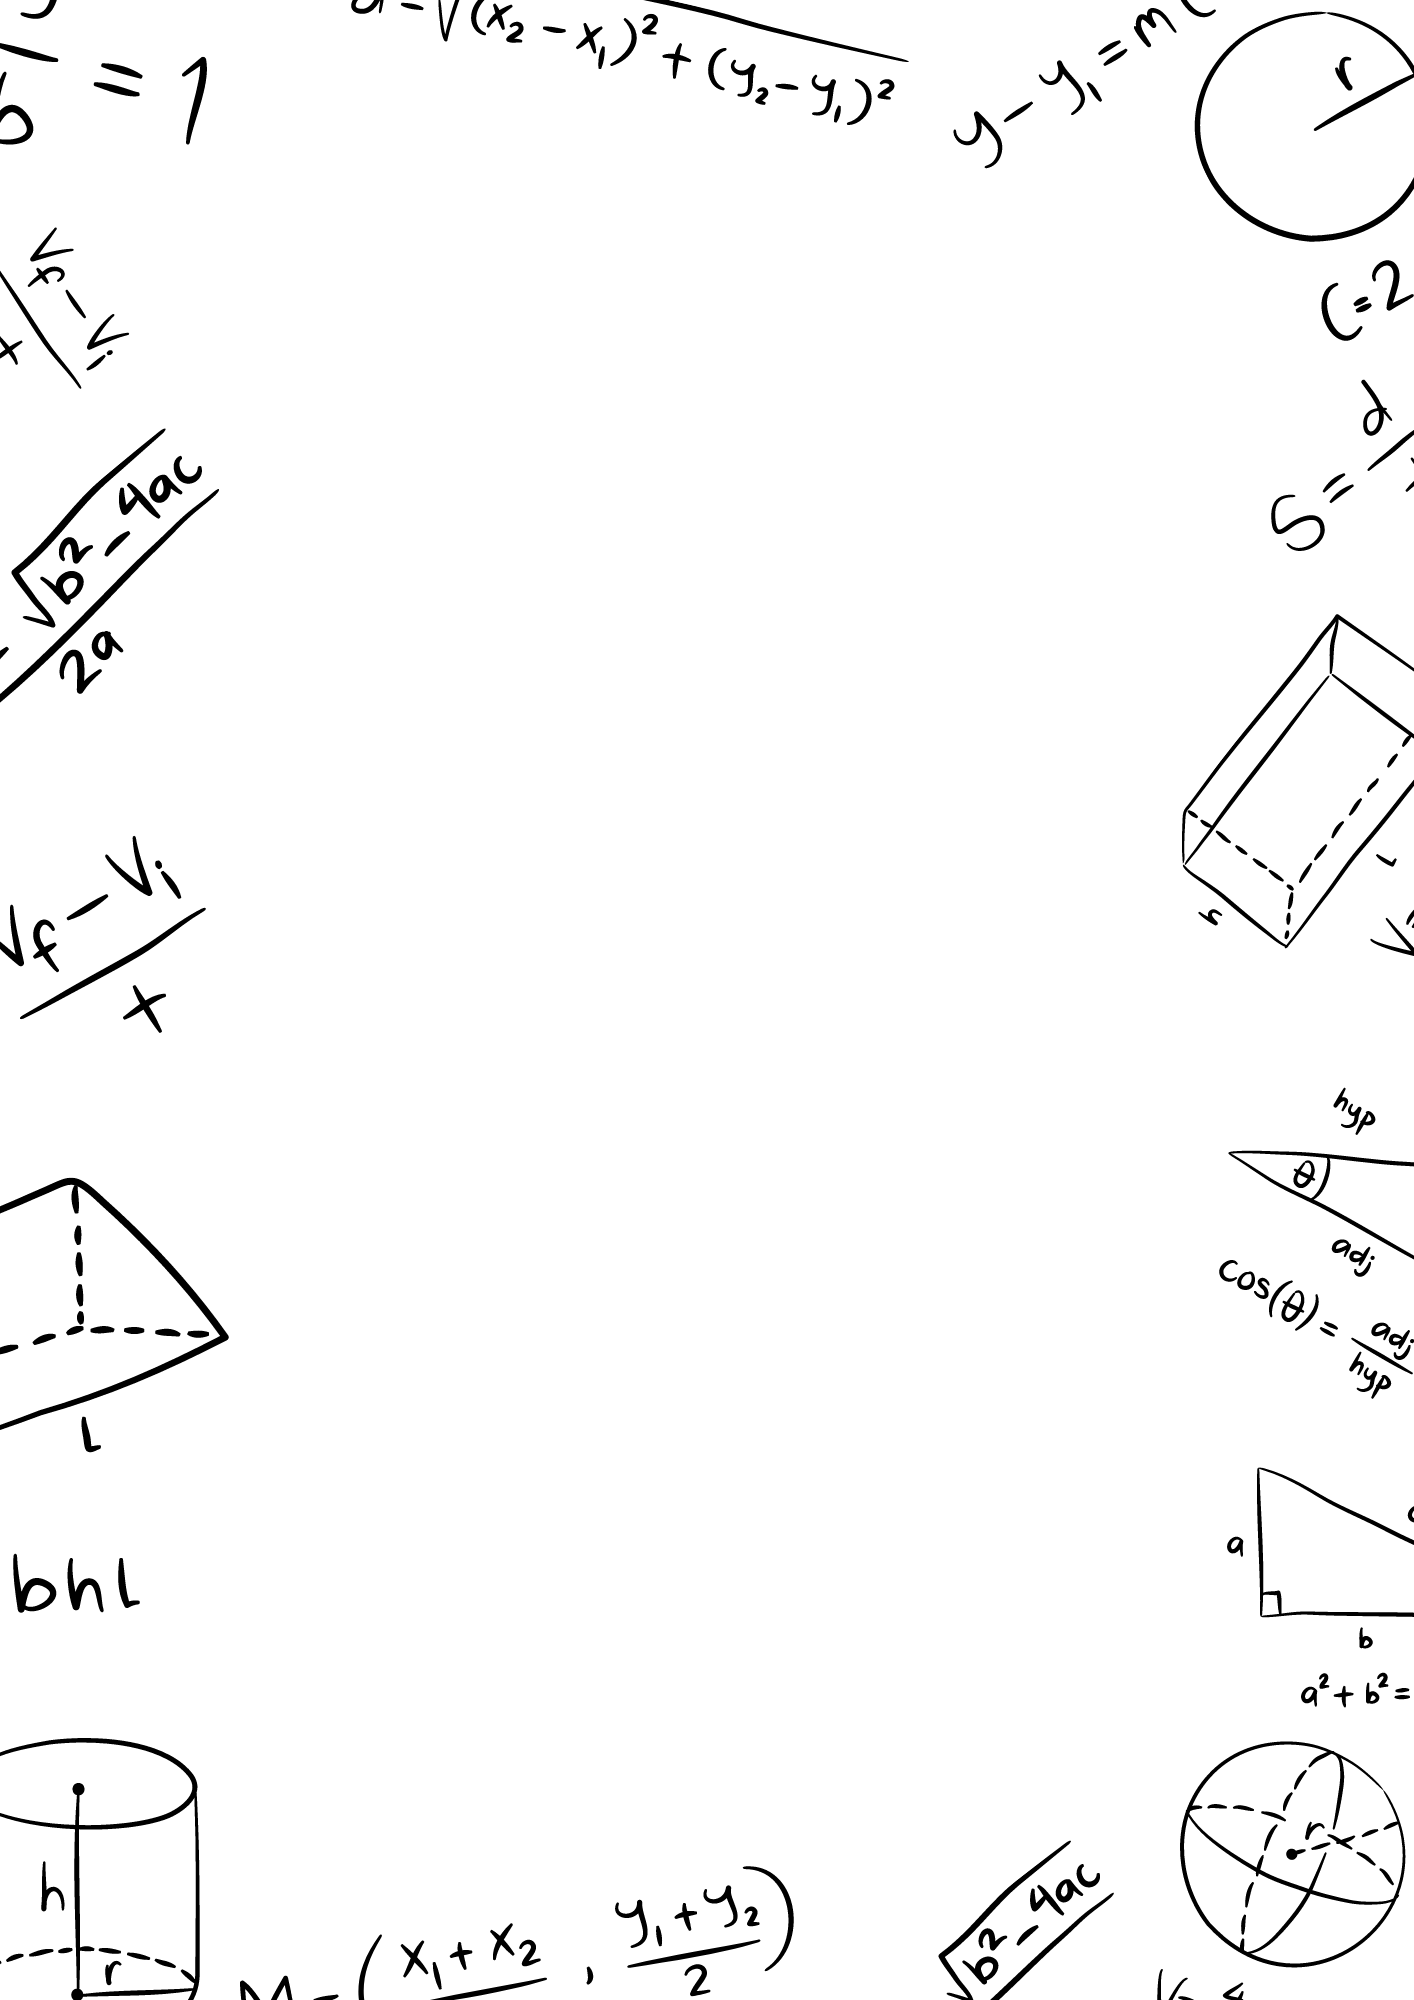
\includegraphics[width=(\paperwidth + 50pt),height=(\paperheight + 50pt)]
        {assets/images/CS215AssignmentCover.png}
    }
}

\maketitle

% \setcounter{tocdepth}{0}
% \tableofcontents

\chapter{Finding Optimal Bandwidth}

\section{Cross-Validation Estimator}

The cross-validation estimator is defined as
\begin{equation*}
    \hat{J}(h) = \int \hat{f}(x)^2 dx - \frac{2}{n}\sum_{i=1}^{n}\hat{f}_{(-i)}
    (X_i), 
\end{equation*}
where $\hat{f}_{(-i)}$ is the histogram estimator after removing the $i$th
observation.

\subsection*{(a)}

We can write the histogram estimator $\hat{f}(x)$ as 
\begin{equation*}
  \begin{aligned}
    \hat{f}(x) &= \sum_{k=1}^{m}\frac{\hat{p_k}}{h}\mathbb{I}    [x\in B_k] \\
    &= \sum_{k=1}^{m}\frac{v_k}{nh}\mathbb{I}[x\in B_k].
  \end{aligned}
\end{equation*} 
Hence,
\begin{equation}
  \begin{aligned}
    \int\hat{f}(x)^2 dx &= \int \left(\sum_{k=1}^{m}\frac{v_k}{nh}\mathbb{I}[x\in
    B_k]\right)^2 dx \\
    &= \sum_{j=1}^{m} \int_{B_j}\left(\sum_{k=1}^{m}\frac{v_k}{nh}\mathbb{I}[x\in
    B_k]\right)^2 dx + 0 \\
    &= \sum_{j=1}^{m}\int_{B_j}\left(\frac{v_j}{nh}\right)^2 dx \\
    &= \sum_{j=1}^{m} \frac{(v_j)^2}{n^2 h^2}h \\
    &= \frac{1}{n^2 h}\sum_{j=1}^{m}(v_j)^2.
  \end{aligned}
  \label{eq1.1}
\end{equation}
This is the required result.

\subsection*{(b)}

Suppose $X_i\in B_j$. Then on removing $X_i$, the number of points in $B_j$ is
$v_j-1$ and the total number of points is $n-1$. Hence, $\hat{f}_{(-i)}(X_i) =
\frac{(v_j-1)}{(n-1)h}$. Using this result, 
\begin{equation}
  \begin{aligned}
    \sum_{i=1}^{n} \hat{f}_{(-i)}(X_i) &= \sum_{i=1}^{n}\sum_{j=1}^{m} \frac{v_j-
    1}{(n-1)h}\mathbb{I}[X_i\in B_j] \\
    &= \sum_{j=1}^{m}\sum_{i=1}^{n} \frac{v_j-1}{(n-1)h}\mathbb{I}[X_i\in B_j] \\
    &= \sum_{j=1}^{m} \frac{v_j-1}{(n-1)h}\cdot v_j \\
    &= \frac{1}{(n-1)h}\sum_{j=1}^{m} (v_j^2 - v_j).
  \end{aligned}
  \label{eq1.2}
\end{equation}
This is the second part. We can combine the \ref{eq1.1} and \ref{eq1.2} parts to
write the cross-validation estimator as 
\begin{equation*}
  \hat{J}(h) = \frac{2}{(n-1)h} - \frac{n+1}{(n-1)h}\sum_{j=1}^{m} \hat{p}_j^2
\end{equation*}

\section{ Using the Cross-Validation Estimator}

\subsection*{(a)}
The probabilities were calculated using \texttt{numpy.histogram} function. The
estimated probabilities $\hat{p}_j$ for all the bins are:
\begin{center}
  \begin{tabular}{ | c | c |}
    \hline
    \textbf{Bin} & \textbf{$\hat{p}_j$} \\
    \hline
    1 & 0.20588235 \\
    2 & 0.48823529 \\
    3 & 0.04705882 \\
    4 & 0.04117647 \\
    5 & 0.13529412 \\
    6 & 0.05882353 \\
    7 & 0.00588235 \\
    8 & 0.0 \\
    9 & 0.01176471 \\
    10 & 0.00588235 \\
    \hline
  \end{tabular}
\end{center}
Using the obtained values, the histogram was plotted using the
\texttt{matplotlib.pyplot.hist} function. The histogram plot can be found in
\texttt{images/10binhistogram.png}.

\begin{figure}[H]
  \centering
  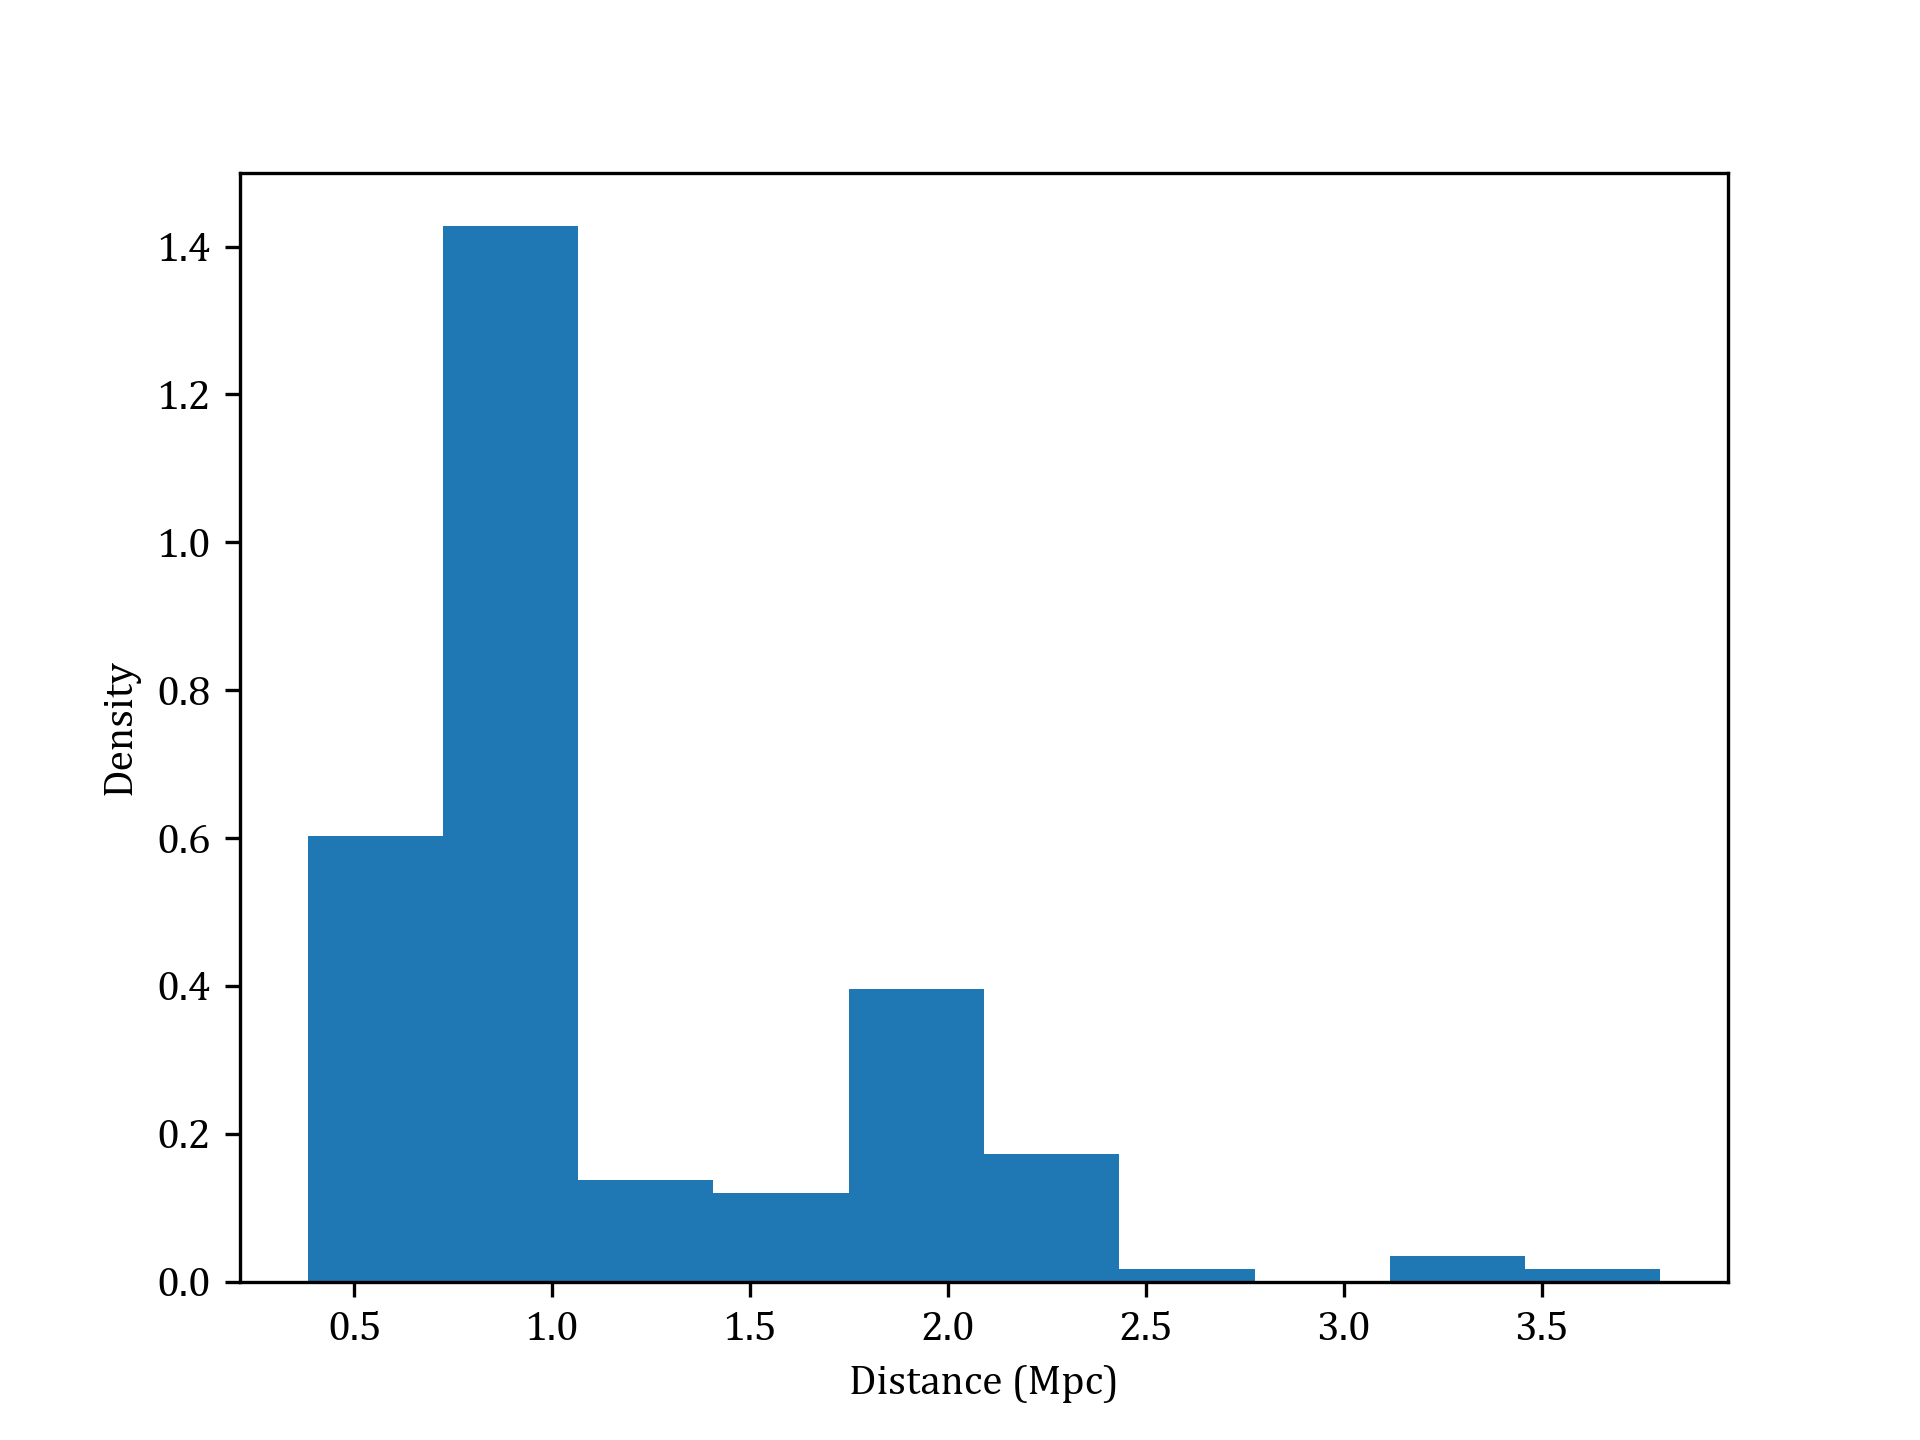
\includegraphics[width=0.5\textwidth]{assets/images/10binhistogram.png}
  \caption{10 Bin Histogram}
\end{figure}


\subsection*{(b)}

The probability distribution is \textbf{oversmoothed}. Lower values of $h$ yield
a lower cross-validation score.

\subsection*{(c)}

The cross-validation score for the number of bins from 1 to 1000 was calculated
using: \texttt{numpy.histogram}, \texttt{numpy.square} and \texttt{numpy.sum}
functions. The plot of cross-validation score versus $h$ can be found in
\texttt{images/crossvalidation.png}

\begin{figure}[H]
  \centering
  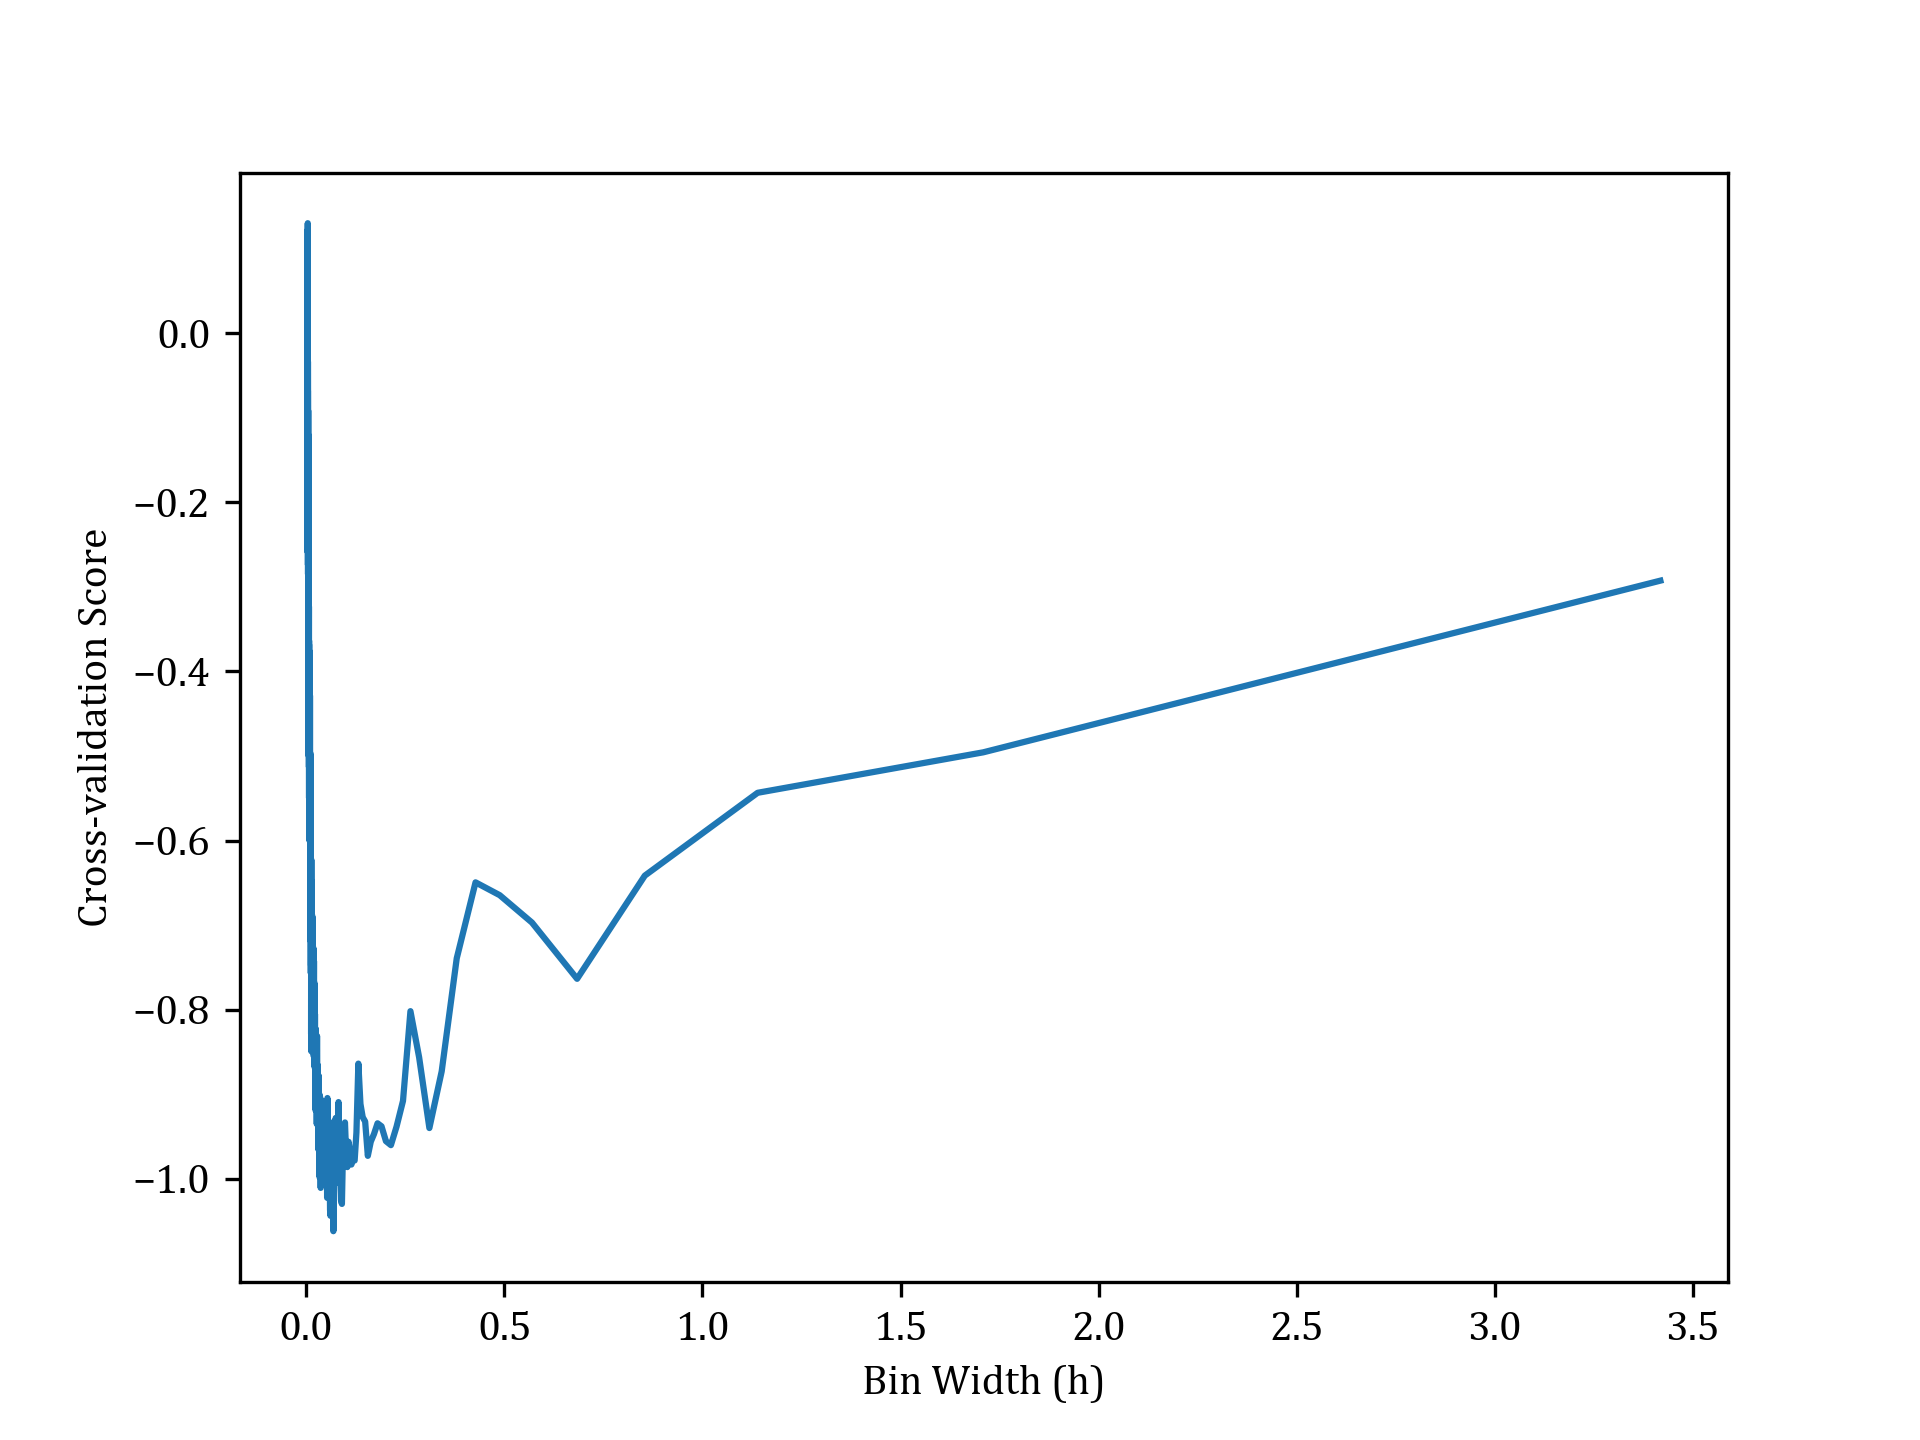
\includegraphics[width=0.5\textwidth]{assets/images/crossvalidation.png}
  \caption{Cross Validation}
\end{figure}

\subsection*{(d)}

The optimal bin width is the value of $h$ for which the cross-validation score is
minimum. From the plot, this corresponded to 50 bins, for which the value of $h$
is \textbf{0.06835999} Mpc.

\subsection*{(e)}

The histogram with optimal value $h^* = 0.06835999$ is present in
\texttt{images/optimalhistogram.png}.

\begin{figure}[H]
  \centering
  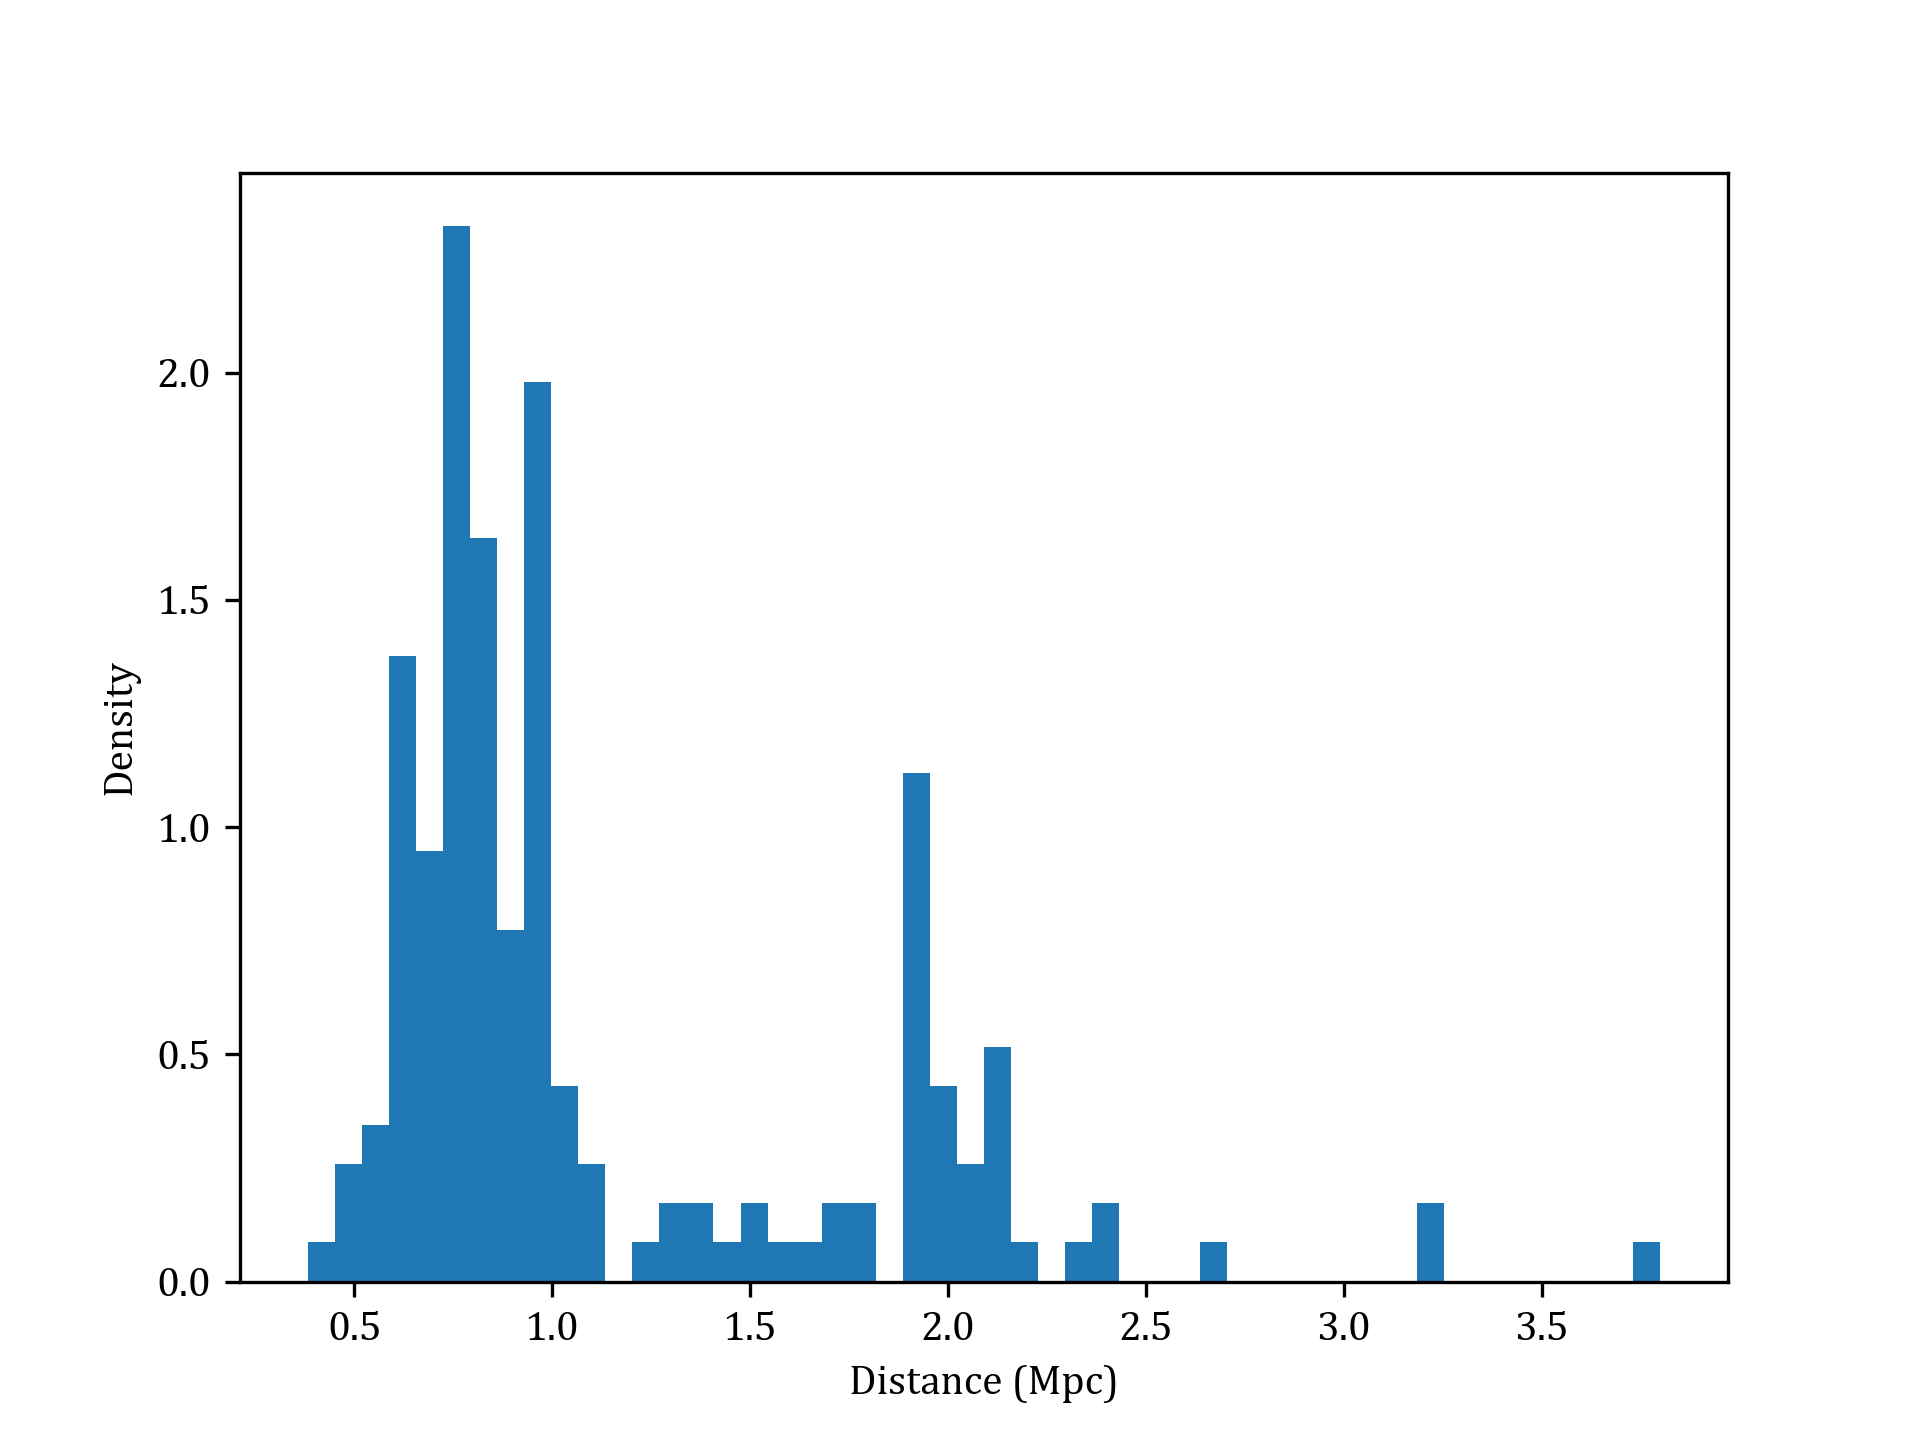
\includegraphics[width=0.5\textwidth]{assets/images/optimalhistogram.png}
  \caption{Cross Validation}
\end{figure}

\subsection*{(f)}

The code for all the parts is present in \texttt{code/1.py}. 

\chapter{Detecting Anomalous Transactions using KDE}

\section{Designing a custom KDE Class}

The implemented code for the class is:

\begin{lstlisting}[caption={2D Epanechnikov KDE class}]
class EpanechnikovKDE:
    def __init__(self, bandwidth=1.0):
        """Initialize with given bandwidth."""
        self.bandwidth = bandwidth
        self.data = None

    def fit(self, data):
        """Fit the KDE model with the provided data."""
        self.data = np.array(data)

    def epanechnikov_kernel(self, x, xi):
        """Epanechnikov kernel function for 2D using vectorized operations."""
        norm_squared = np.sum(((xi - x) / self.bandwidth) ** 2, axis=-1)
        return ((2 / np.pi) * (1 - norm_squared)) * (norm_squared <= 1)

    def evaluate(self, x):
        """Evaluate the KDE at multiple points x in 2D."""
        return self.epanechnikov_kernel(x, self.data).mean() / (self.bandwidth ** 2)
\end{lstlisting}

\section{Estimating Distribution of Transactions}
For the distribution that is obtained from the given data, we have 2 modes.
The 3D graph for the given data is as follows:

\begin{figure}[H]
  \centering
  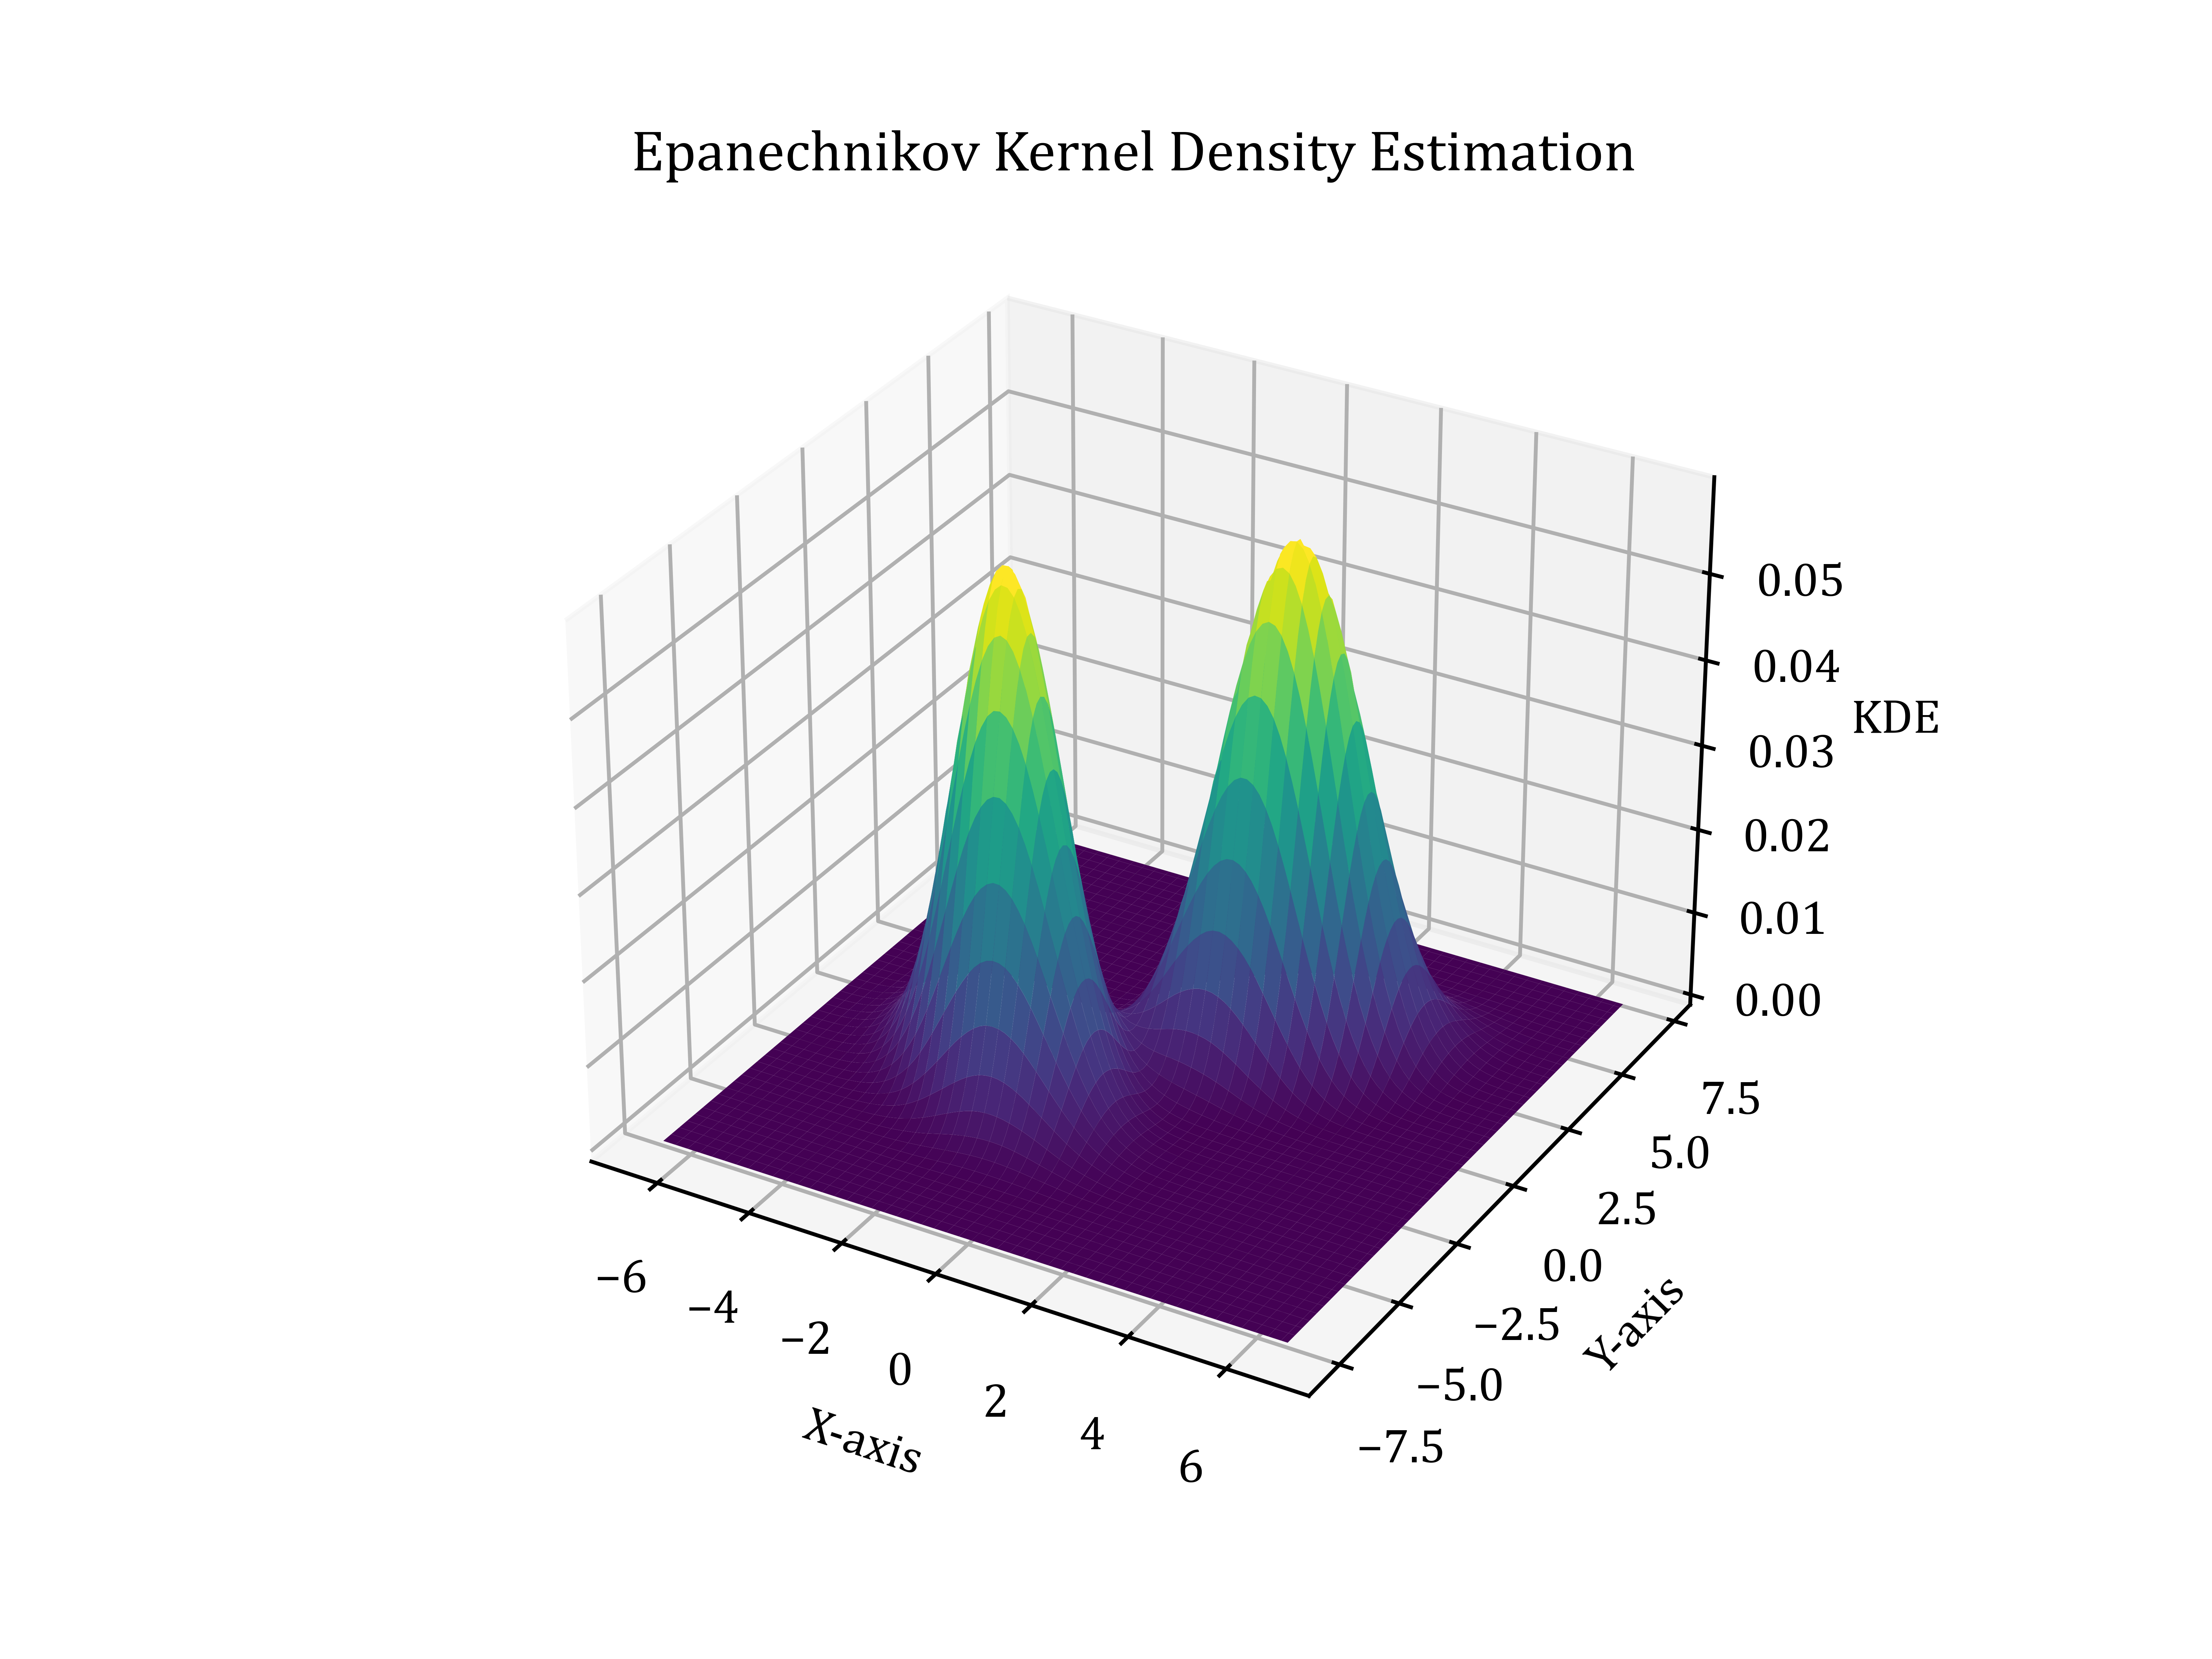
\includegraphics[width=0.4\textwidth]
  {assets/images/transaction_distribution.png}
  \caption{Transaction Distribution}
\end{figure}
\chapter{Higher-Order Regression}

\section{Showing that the Point \texorpdfstring{$(\bar{x}, \bar{y})$}{(x-bar, y
bar)} lies on the Least-Squares Regression Line}
In simple linear regression, the model is given by:
\begin{equation*}
    Y = \beta_0 + \beta_1 x + \epsilon
\end{equation*}
Where:
\begin{itemize}
    \setlength{\itemsep}{-2pt}
    \item $\beta_0$ is the intercept,
    \item $\beta_1$ is the slope, and
    \item $\epsilon$ is the error term.
\end{itemize}
The least squares regression line, which minimizes the sum of squared residuals,
is given by the following equation:
\begin{equation*}
    \hat{Y} = \hat{\beta}_0 + \hat{\beta}_1 x
\end{equation*}
To find the least-squares estimates $\hat{\beta}_0$ and $\hat{\beta}_1$, we have
to minimize the sum of squared residuals (SSR):
\begin{equation*}
\text{SSR} = \sum_{i=1}^{n} \left( y_i - (\hat{\beta}_0 + \hat{\beta}_1 x_i)
\right)^2
\end{equation*}
Partial derivative with respect to $\hat{\beta}_0$:
\begin{equation*}
    \begin{aligned}
        \frac{\partial \text{SSR}}{\partial \hat{\beta}_0} &= -2 \sum_{i=1}^{n}
        \left( y_i - \hat{\beta}_0 - \hat{\beta_1} x_i \right) = 0 \\
        \sum_{i=1}^{n} y_i &= n \hat{\beta}_0 + \hat{\beta}_1 \sum_{i=1}^{n} x_i
        \\
        \hat{\beta}_0 &= \bar{y} - \hat{\beta}_1 \bar{x} \\
    \end{aligned}
\end{equation*}
Partial derivative with respect to $\hat{\beta}_1$:
\begin{equation*}
    \begin{aligned}
        \frac{\partial \text{SSR}}{\partial \hat{\beta}_1} &= -2 \sum_{i=1}^{n}
        x_i \left( y_i - \hat{\beta}_0 - \hat{\beta}_1 x_i \right) = 0 \\
        \sum_{i=1}^{n} x_i y_i &= \hat{\beta_0} \sum_{i=1}^{n} x_i +
        \hat{\beta_1} \sum_{i=1}^{n} x_i^2 \\
        \hat{\beta_1} &= \frac{\sum_{i=1}^{n} (x_i - \bar{x})(y_i - \bar{y})}
        {\sum_{i=1}^{n} (x_i - \bar{x})^2} \\
    \end{aligned}
\end{equation*}
Now, substituting $\bar{x}$ into the regression line equation gives
\begin{equation*}
\hat{Y} = \hat{\beta}_0 + \hat{\beta}_1 \bar{x}
\end{equation*}
Substitute $\hat{\beta}_0 = \bar{y} - \hat{\beta}_1 \bar{x}$:
\begin{equation*}
\hat{Y} = (\bar{y} - \hat{\beta}_1 \bar{x}) + \hat{\beta}_1 \bar{x}
\end{equation*}
Simplifying this:
\begin{equation*}
    \hat{Y} = \bar{y}
\end{equation*}
Thus, the point $(\bar{x}, \bar{y})$ lies exactly on the least-squares regression
line.

\section{New model using \texorpdfstring{$z = x - \bar{x}$}{z = x - x-bar}}

The original least-squares estimate for $\beta_1$:

\begin{equation*}
    \hat{\beta}_1 = \frac{\sum (x_i - \bar{x})(y_i - \bar{y})}{\sum (x_i -\
    \bar{x})^2}
\end{equation*}
Since $z_i = x_i - \bar{x}$, this can be rewritten in terms of $z$:

\begin{equation*}
    \hat{\beta}_1^* = \frac{\sum z_i (y_i - \bar{y})}{\sum z_i^2}
\end{equation*}
The original least squares estimate for $\beta_0$:

\begin{equation*}
    \hat{\beta}_0 = \bar{y} - \hat{\beta}_1\bar{x}
\end{equation*}
For the intercept in the new model, we know that $z$ is centered around 0,
which means $\bar{z} = 0$. Therefore, the least squares estimate of $\beta_0^*$
is simply the average of $y$, i.e., $\bar{y}$:

\begin{equation*}
    \hat{\beta}_0^* = \bar{y}
\end{equation*}
Since $z = x - \bar{x}$, this is just a change in the predictor variable.
Therefore, the slope of the regression line does not change, and we have the
following:

\begin{equation*}
\hat{\beta}_1^* = \hat{\beta}_1
\end{equation*}
In the new model, the least squares estimates of $\beta_0$ are:

\begin{equation*}
\hat{\beta}_0^* = \bar{y}
\end{equation*}
On the other hand, in the original model, the least squares estimate of $\beta_0$
is:

\begin{equation*}
\hat{\beta}_0 = \bar{y} - \hat{\beta}_1 \bar{x}
\end{equation*}
Thus, the relationship between $\beta_0$ and $\beta_0^*$ is:

\begin{equation*}
\hat{\beta}_0^* = \hat{\beta}_0 + \hat{\beta}_1 \bar{x}
\end{equation*}

\noindent \textbf{Model Differences:}
The original model estimates both the intercept and slope based on uncentered
values of $x$, while the transformed model estimates the intercept at the mean of
$Y$ and uses a centered version of $x$ (now $z$). The slope remains the same in
both models.

\noindent \textbf{Interpretation Differences:}
The intercept in the original model reflects the value of $Y$ when $x$ is zero
(or of a different origin), while in the new model, it represents the mean of
$Y$ at the mean of $x$, providing a different baseline from which predictions are
made.

\section{Regression for a Dataset}

\begin{figure}[H]
  \centering
  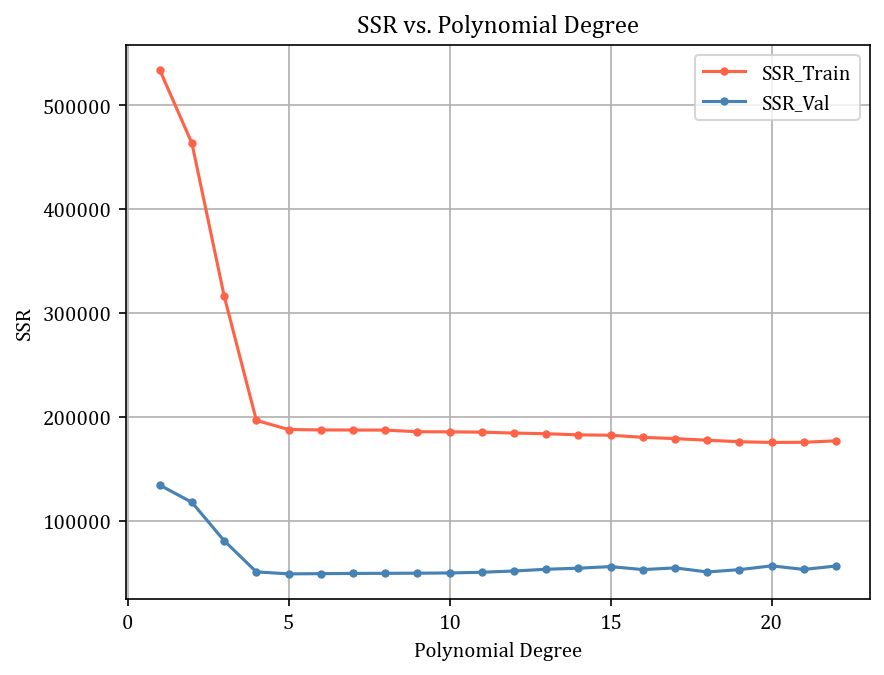
\includegraphics[width=0.3\textwidth]{assets/images/SSR-graph.png}
  \caption{The SSR graph for various degrees}
\end{figure}

By the SSR graph above, degree = 5 seems to be the optimal degree for the
polynomial.

\subsection{Correct Fit}
\begin{figure}[H]
  \centering
  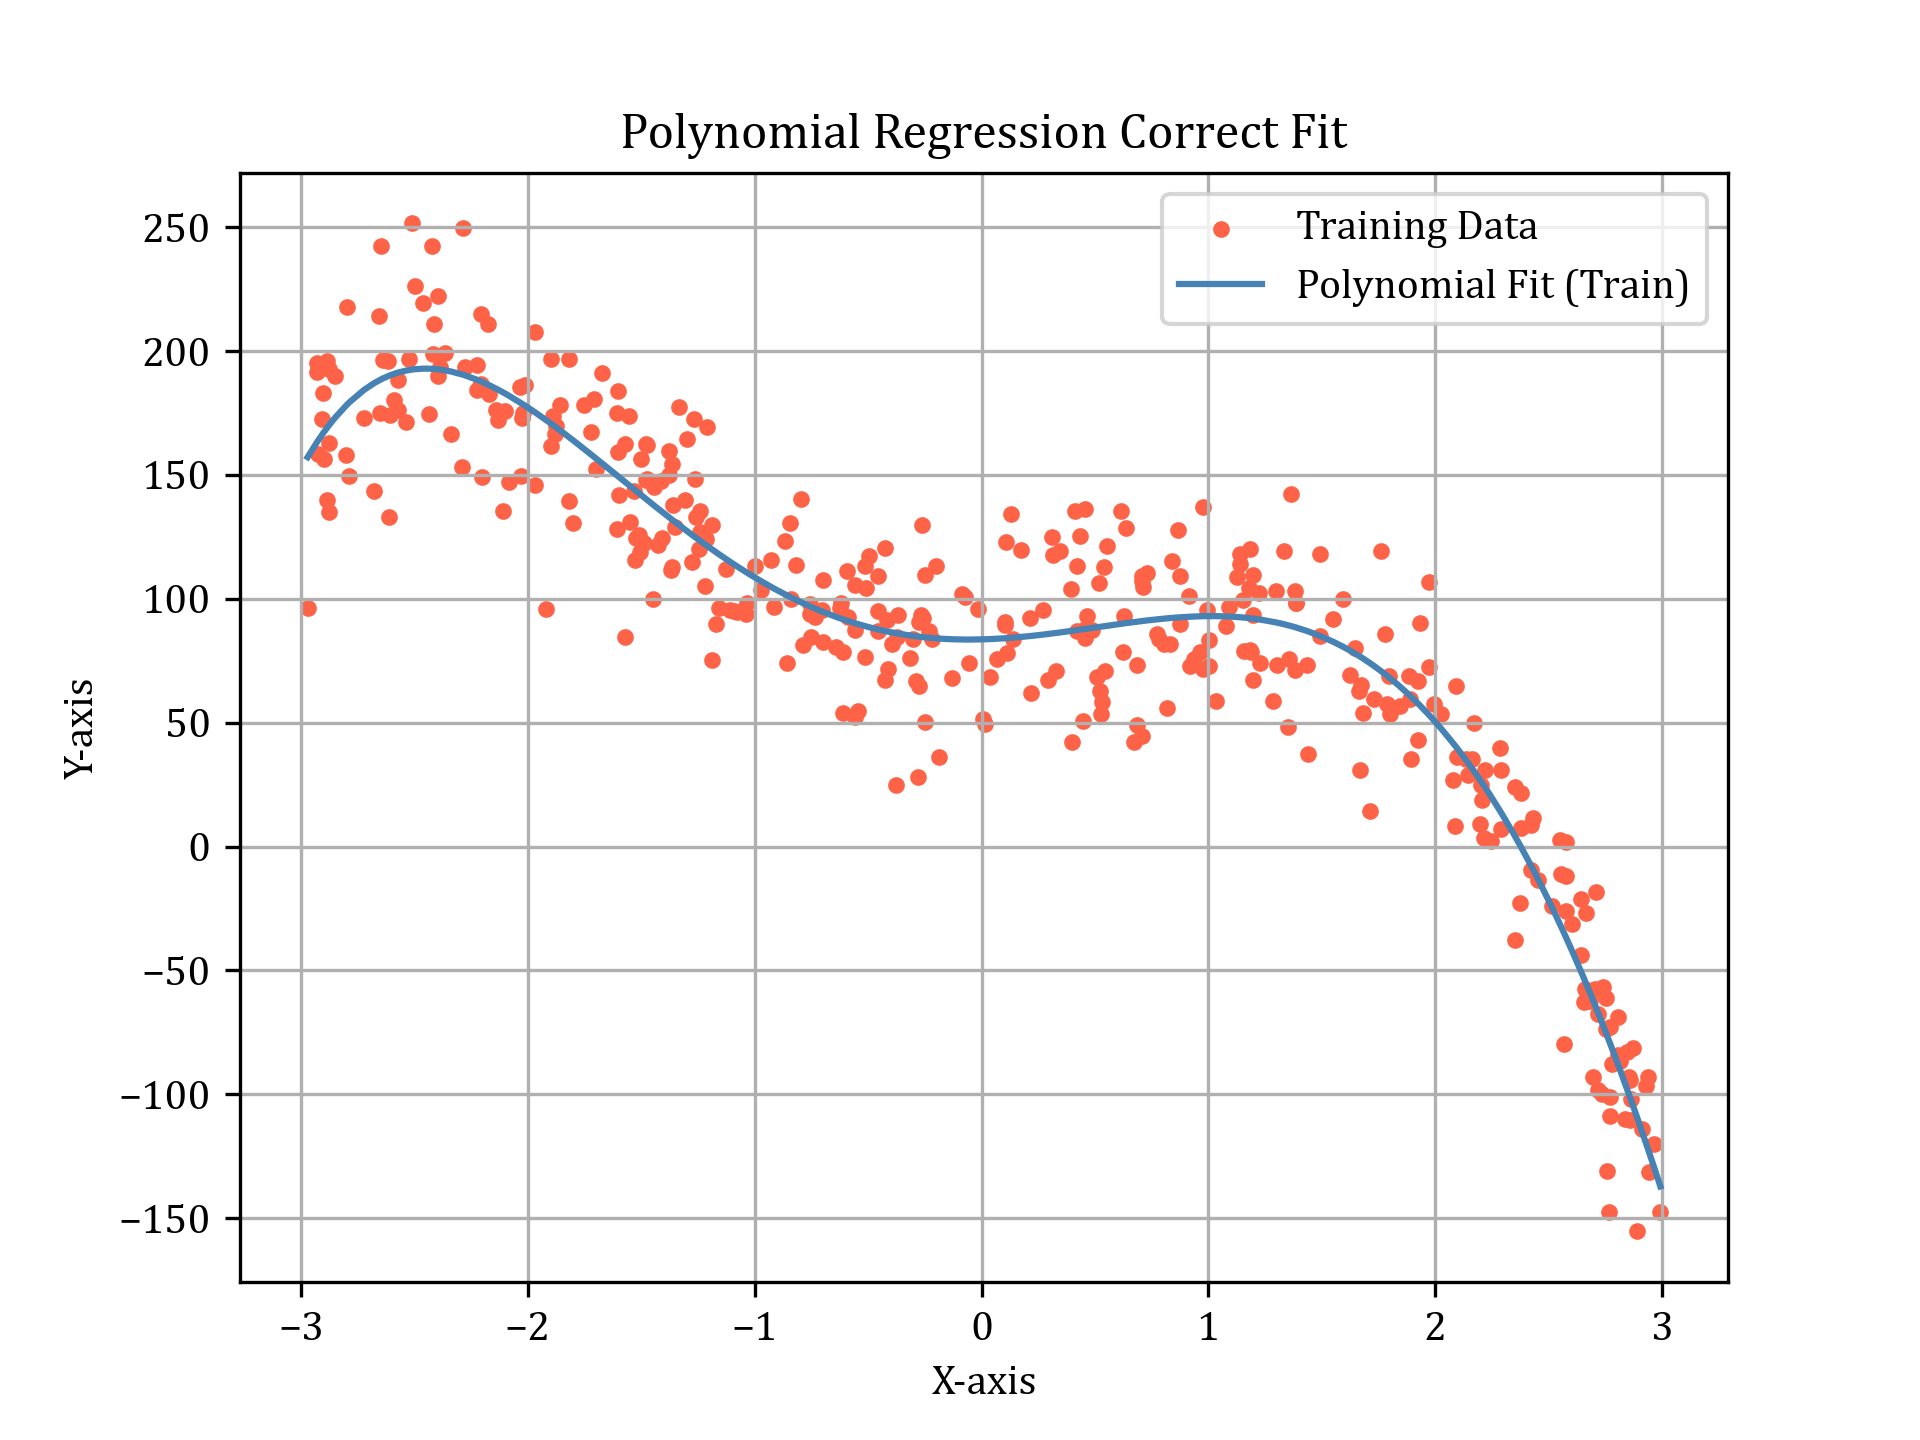
\includegraphics[width=0.4\textwidth]{assets/images/3_correctfit.png}
  \caption{Correct Fit at degree = 5}
\end{figure}

\subsection{UnderFit}
\begin{figure}[H]
  \centering
  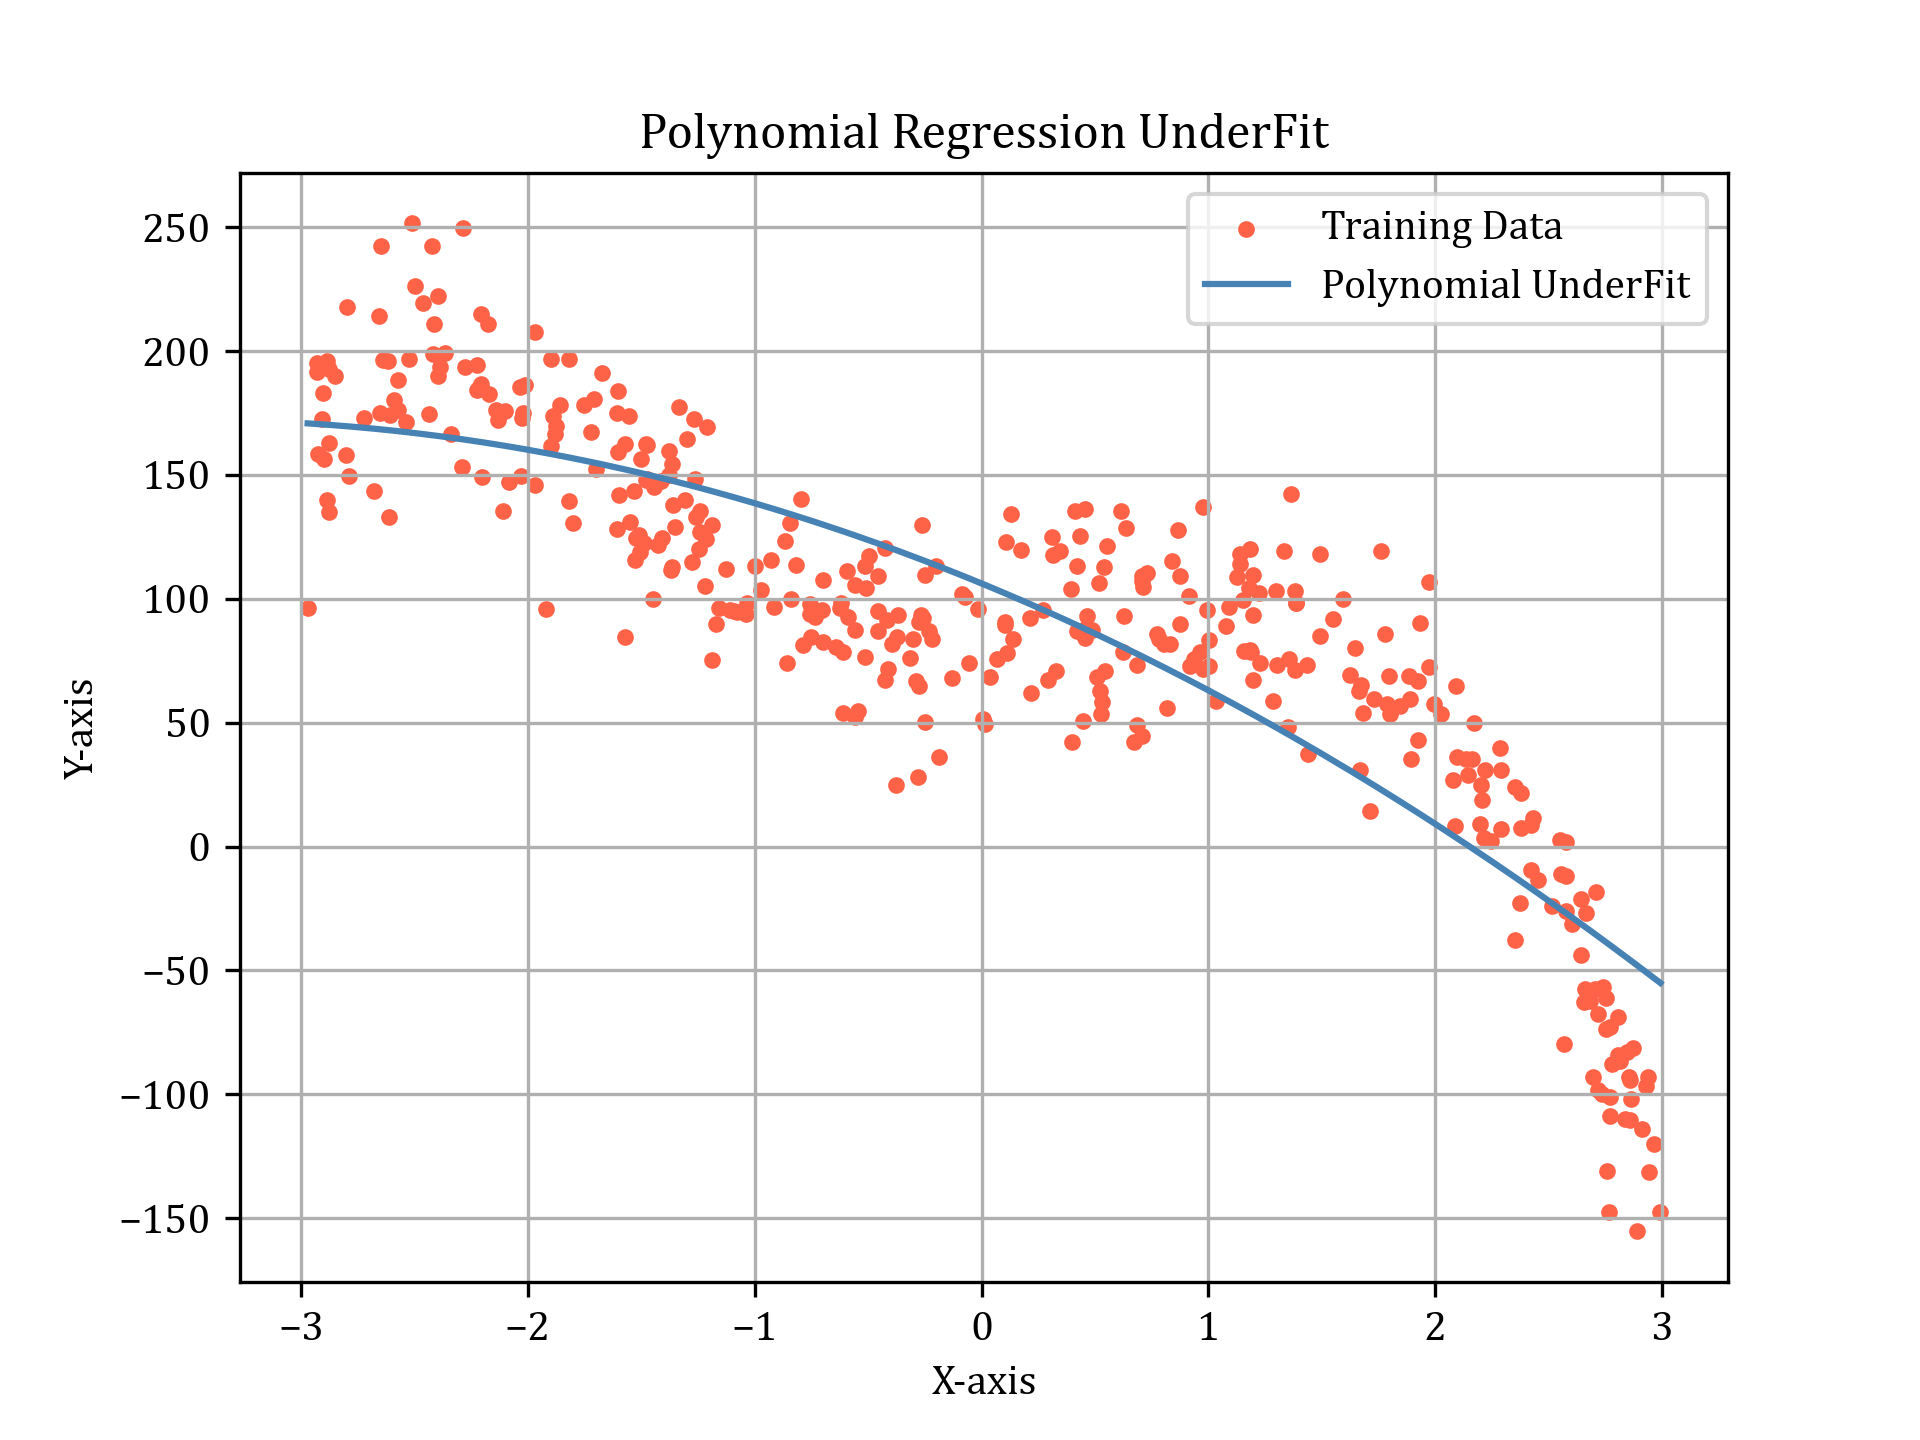
\includegraphics[width=0.4\textwidth]{assets/images/3_underfit.png}
  \caption{UnderFit at degree = 2}
\end{figure}

\subsection{OverFit}
\begin{figure}[H]
  \centering
  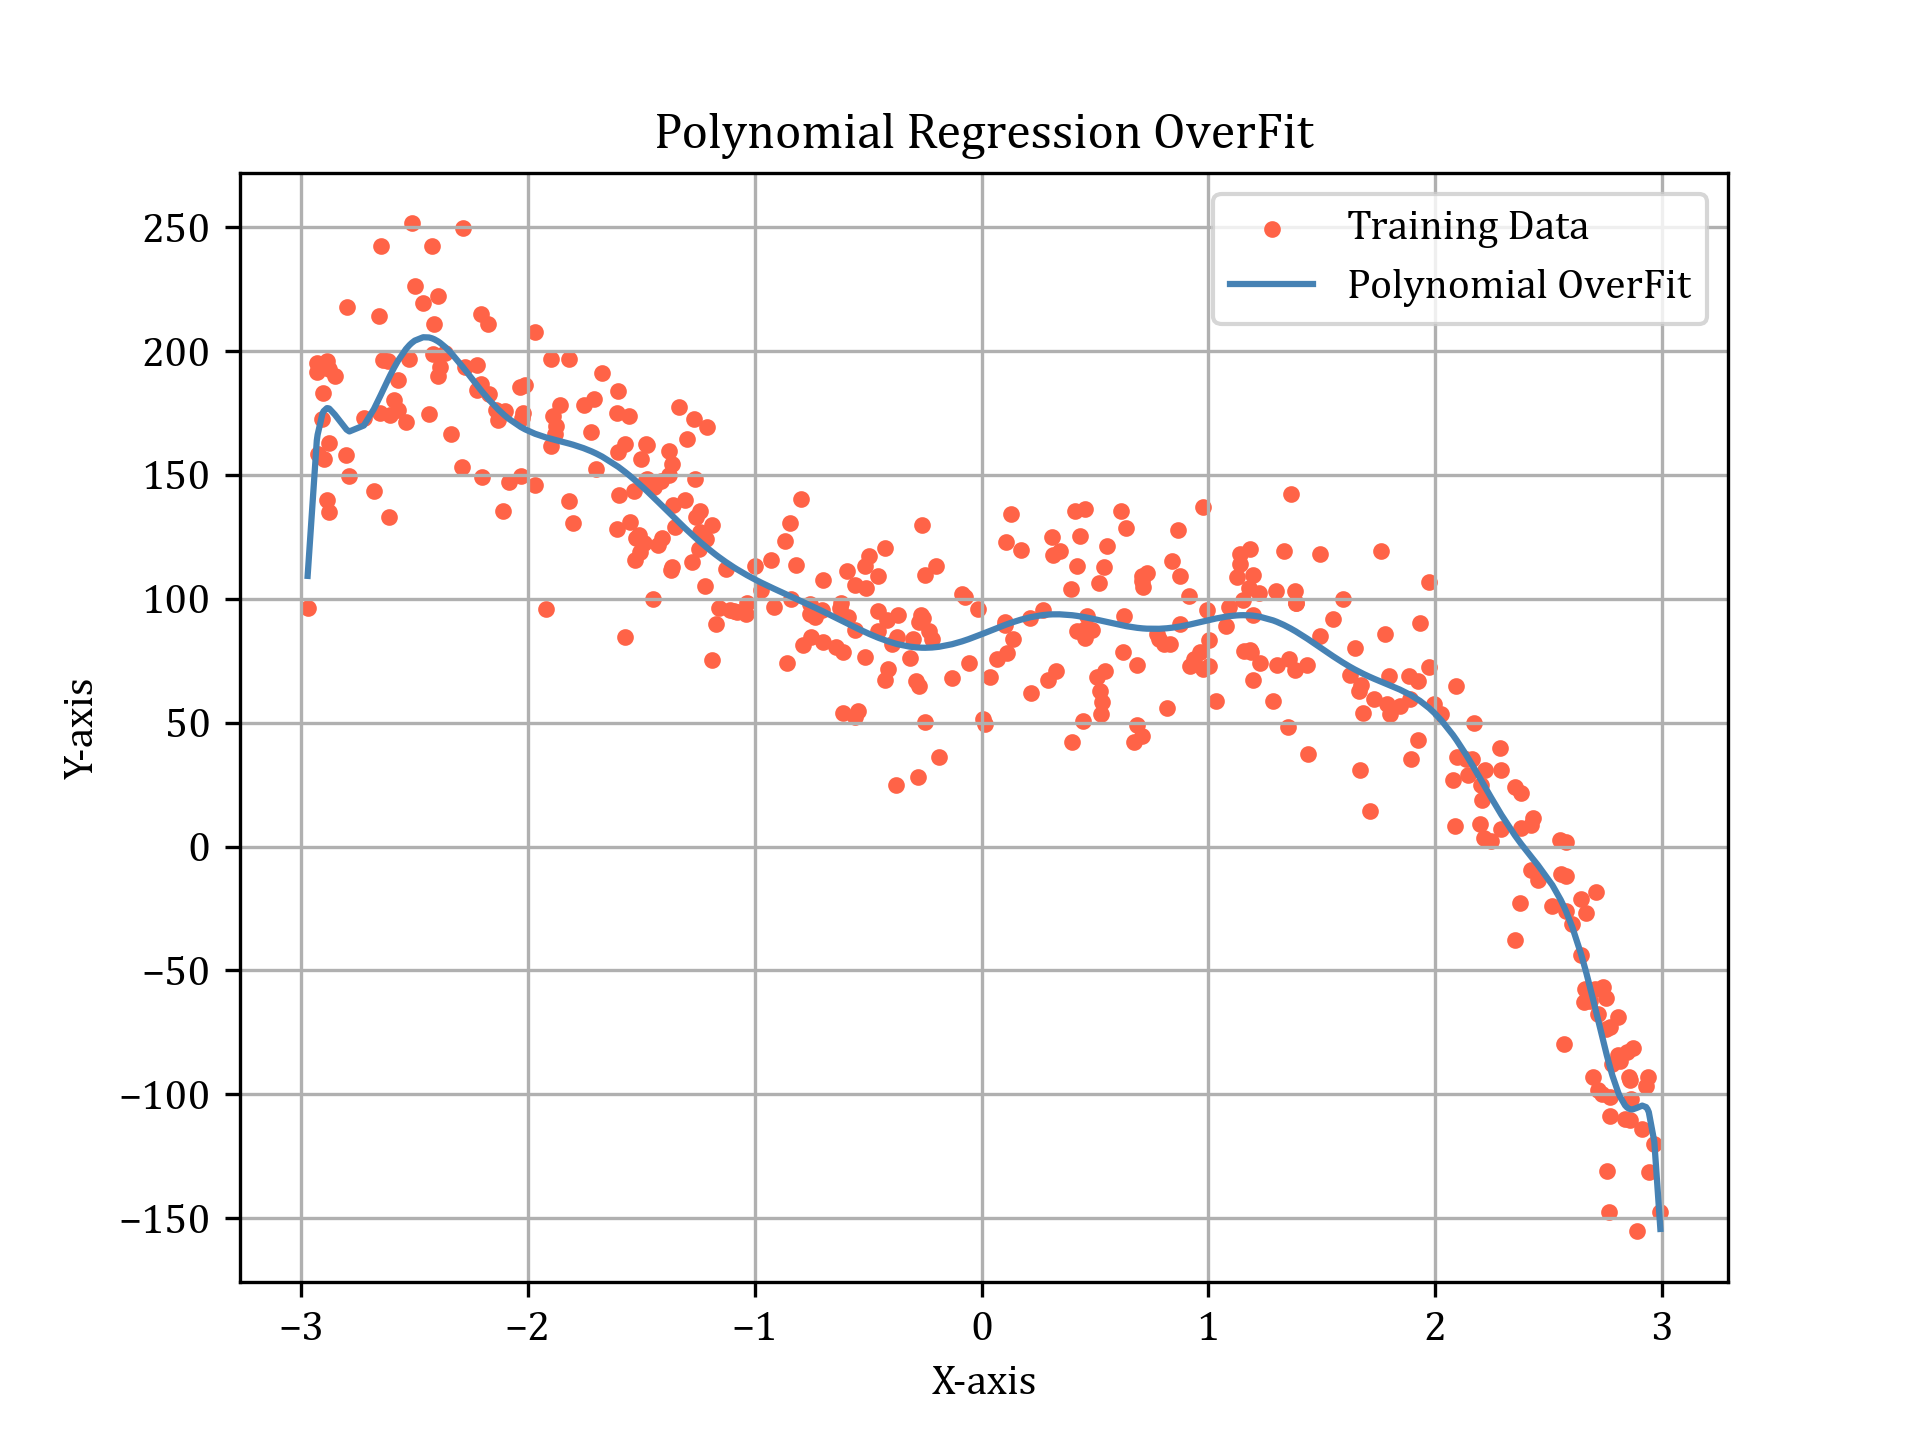
\includegraphics[width=0.4\textwidth]{assets/images/3_overfit.png}
  \caption{OverFit at degree = 20}
\end{figure}

\chapter{Quality in Inequalities}

\begin{tcolorbox}[title=]
    Let us dive deeper into the inequalities we have studied in class (and a new
    one):

    \vspace{10pt}
    \begin{mdframed}[backgroundcolor=lightblue, linecolor=blue, linewidth=1.5pt]
        \textbf{Definition 5 (Markov's Inequality).}
        \textit{Let $X$ be any non-negative random variable and $a > 0$,}
        
        \begin{equation*}
            \text{P}[X \ge a] \le \dfrac{\mathbb{E}[X]}{a}.
        \end{equation*}
    \end{mdframed}
\end{tcolorbox}

\section*{\colS{$\S$} Task A \hfill \normalfont \large [1+2]}

\begin{tcolorbox}
    Give an intuitive \enquote{proof} for this inequality and a reason why it
    could be correct (you can try playing around with different $ X$'s and $a$'s).
    
    Now, prove this inequality rigorously using continuous random variables. Try
    to reason about the definition of expectation and how you can manipulate it
    to serve your purpose.
\end{tcolorbox}

% Solution A

The variable $X$ is a non-negative random variable. Hence, there is a lower bound
on the value that $X$ can take. Intuitively, for a given expected value
$\mathbb{E}[X]$, there must also be a upper bound on the probability of $X$
taking a large value.

Let us look at the rigorous proof. Consider a continuous random variable $x$ with
pdf $f(x)$, and let $a>0$. The expected value is defined as

\begin{equation*}
    \begin{aligned}
        \mathbb{E}[x] &= \int_{0}^{\infty}xf(x)dx \\
        &= \int_{0}^{a}xf(x)dx + \int_{a}^{\infty}xf(x)dx \\
        &\ge \int_{0}^{a}0\cdot f(x)dx + \int_{a}^{\infty}a\cdot f(x)dx \\
        &\ge 0+a\int_{a}^{\infty}f(x)dx.
    \end{aligned}
\end{equation*}

Now, $P[x\ge a]=\int_{a}^{\infty}f(x)dx$. Hence,

\begin{equation*}
    \begin{aligned}
        \mathbb{E}[x] &\ge a\cdot P[x\ge a] \\
        \implies P[x\ge a] &\le \frac{\mathbb{E}[x]}{a}.
    \end{aligned}
\end{equation*}

Hence, Markov's inequality holds.

\section*{\colS{$\S$} Task B \hfill \normalfont \large [4]}

\begin{tcolorbox}
    Now that we have established this inequality, let us move on to linking it to
    what we have already studied in class is the Chebyshev-Cantelli inequality.

    Use Markov's inequality to prove the following version of the Chebyshev
    Cantelli inequality for a random variable $X$ with mean $\mu$ and variance
    $\sigma^2$: for every $\tau > 0$, we have

    \begin{equation*}
        \text{P}[(x - \mu) \ge \tau] \le \dfrac{\sigma^2}{\sigma^2 + \tau^2}.
    \end{equation*}
\end{tcolorbox}

% Solution B

Let $X$ be any random variable with mean $\mu$ and variance $\sigma^2$. Consider
a new random variable $Y = X-\mu$. Then $\mathbb{E}[Y]=0$ and $Var[Y]=\sigma^2$.
Let $\tau>0$ be a number. Let $t$ be a number such that $t+\tau>0$. Then

\begin{equation*}
    \begin{aligned}
        \Pr[Y \geq \tau] &= \Pr[Y + t \geq \tau + t] \\
        &= \Pr\left[\left(\frac{Y+t}{\tau+t}\right)\geq 1\right] \\
        &\le \Pr\left[\left(\frac{Y+t}{\tau+t}\right)^2\geq 1\right]
    \end{aligned}
\end{equation*}

Using Markov's inequality on the non-negative random variable
$\frac{Y+t}{\tau+t}$, we get

\begin{equation*}
    \begin{aligned}
        \Pr[Y\ge\tau] &\le \mathbb{E}\left[\left(\frac{Y+t}
        {\tau+t}\right)^2\right] \\
        &\le \frac{\mathbb{E}[(Y+t)^2]}{(\tau+t)^2} \\
        &\le \frac{\mathbb{E}[Y^2]+0+t^2}{(\tau+t)^2} \\
        &\le \frac{0+\sigma^2+t^2}{(\tau+t)^2}.
    \end{aligned}
\end{equation*}

Hence, the inequality

\begin{equation*}
    \Pr[Y\ge\tau]\le \frac{\sigma^2+t^2}{(\tau+t)^2}
\end{equation*}

should hold for any $t$ such that $t+\tau>0$. It can be shown that the RHS is
minimized for $t=\frac{\sigma^2}{\tau}$. Also, $\tau+t\ge 0$ in this case. Hence

\begin{equation*}
    \begin{aligned}
        \Pr[X-\mu>\tau] &\le \frac{\sigma^2+\frac{\sigma^4}{\tau^2}}
        {\left(\tau+\frac{\sigma^2}{\tau}\right)^2} \\
        &\le \sigma^2\frac{\tau^2+\sigma^2}{(\tau^2+\sigma^2)^2} \\
        &\le \frac{\sigma^2}{\sigma^2+\tau^2}.
    \end{aligned}
\end{equation*}

Hence, Chebyshev-Cantelli inequality holds.

\section*{\colS{$\S$} Task C \hfill \normalfont \large [3]}

\begin{tcolorbox}
    Yay, our inequalities are successfully linked! Now we can move on to proving a
    strong bound through these inequalities... start by showing that for a
    random variable $X$ where $M_X(t)$ represents the MGF (see Question 1) for
    $X$, the following hold:

    \begin{equation*}
        P[X \ge x] \le e^{-tx} M_X(t) \ \forall t > 0.
    \end{equation*}
    \begin{equation*}
        P[X \le x] \le e^{-tx} M_X(t) \ \forall t < 0.
    \end{equation*}
\end{tcolorbox}

% Solution C

The MGF is defined by $M_X(t) = \mathbb{E}[e^{tX}]$. Now, for $t>0$,

\begin{equation*}
    \begin{aligned}
        \Pr[X\ge x] &= \Pr[tX\ge tx] \\
        &= \Pr[e^{tX}\ge e^{tx}].
    \end{aligned}
\end{equation*}

Now, using Markov's inequality on the random variable $e^{tX}$, we get

\begin{equation*}
    \Pr[e^{tX}\ge e^{tx}] \le \mathbb{E}[e^{tX}]\cdot e^{-tx}.
\end{equation*}

Hence, using the definition of MGF,

\begin{equation}
    \Pr[X\ge x] \le e^{-tx}M_X(t) \, \forall t>0.
    \label{e4.1}
\end{equation}

Similarly, for $t<0$,

\begin{equation*}
    \begin{aligned}
        \Pr[X\le x] &= \Pr[tX\ge tx] \\
        &= \Pr[e^{tX} \ge e^{tx}].
    \end{aligned}
\end{equation*}

Using Markov's inequality and the definition of MGF, we get

\begin{equation*}
        \Pr[e\le x] \le \mathbb{E}[e^{tX}]e^{-tx}.
\end{equation*}

Hence,

\begin{equation}
    \Pr[X\le x] \le e^{-tx}M_X(t) \, \forall t<0.
    \label{e4.2}
\end{equation}

The required inequalities are \ref{e4.1} and \ref{e4.2}.

\section*{\colS{$\S$} Task D ($\star$) \hfill \normalfont \large [1+4+1]}

\begin{tcolorbox}
    Now take $n$ \textbf{independent} Bernoulli random variables $X_1, X_2,
    \ldots, X_n$ where $\mathbb{E}[X_i] = p_i$. Since each $X_i$ has the same
    distribution and is independent of all other $X_j's$, we call the collection
    of random variables $X_1, \ldots, X_n$ a collection of \textit{independent}
    and \textit{identically distributed} (i.i.d) random variables.
    
    Let us define a new random variable $Y$ as the sum of these random variables
    that is, $Y = \sum_{i = 1}^n X_i$.

    \vspace{10pt}
    \begin{enumerate}
        \item What is the expectation of $Y$?
        \item Show that

            \begin{equation*}
                P[Y \ge (1 + \delta) \mu] \le
                \dfrac{e^{\mu(e^t - 1)}}{e^{(1 + \delta) t \mu}}
            \end{equation*}

        \item Show how to improve this bound further by choosing an appropriate
        value of $t$.
    \end{enumerate}
\end{tcolorbox}

% Solution D

Take $n$ independent Bernoulli random variables $X_1, X_2, \ldots, X_n$ where
$\mathbb{E}[X_i]=p_i$. Since the random variables are given to be identically
distributed, let $p=p_i$. Define random variable $Y=\sum_{i=1}^{n}X_i$.

\subsection*{1}

The expected value of $Y$ is 

\begin{equation*}
    \begin{aligned}
        \mathbb{E}[Y] &= \mathbb{E}\left[\sum_{i=1}^{n}X_i\right] \\
        &= \sum_{i=}^{n}\mathbb{E}[X_i] \\
        &= \sum_{i=1}^{n}p_i \\
        &= np.
    \end{aligned}
\end{equation*}
Hence, $\mu=\mathbb{E}[Y]=np$.

\subsection*{2}

Since $X_i$ are independent, the MGF of $Y$ is given by

\begin{equation*}
    \begin{aligned}
        M_Y(t) &= \mathbb{E}[e^{tY}] \\
        &= \mathbb{E}[e^{t(X_1+\cdots+X_n)}] \\
        &= \left(\mathbb{E}[e^{tX}]\right)^n \\
        &= (M_X(t))^n
    \end{aligned}
\end{equation*}
where $X$ is a Bernoulli random variable. Using \ref{e1.2} with $z=e^t$, we get

\begin{equation*}
    \begin{aligned}
        M_X(t) &= 1-p +pe^t \\
        &= 1+p(e^t-1) \\
        &\le e^{p(e^t-1)}
    \end{aligned}
\end{equation*}
since $e^x-x-1\ge 0\ \forall x\in\mathbb{R}$. Using this result,

\begin{equation*}
    \begin{aligned}
        M_Y(t) &\le \left(e^{p(e^t-1)}\right)^n \\
        &\le e^{np(e^t-1)} \\
        &\le e^{\mu(e^t-1)}.
    \end{aligned}
\end{equation*}
Now, we will use the inequality \ref{e4.1} proven in Task C. For $t>0$ and any
$\delta$,

\begin{equation*}
    \begin{aligned}
        \Pr[Y\ge (1+\delta)\mu] &\le \frac{M_Y(t)}{e^{(1+\delta)t\mu}} \\
        &\le \frac{e^{\mu(e^t-1)}}{e^{(1+\delta)t\mu}}.
    \end{aligned}
\end{equation*}
Hence, the result is proved.
 
\subsection*{3}
Using calculus, it can be shown that the expression

\begin{equation*}
    \frac{e^{\mu(e^t-1)}}{e^{(1+\delta)t\mu}}
\end{equation*}
attains its minimum value when $e^t=1+\delta$, i.e.,

\begin{equation*}
    \begin{aligned}
        \Pr[Y\ge (1+\delta)\mu] &\le \frac{e^{\mu((1+\delta)-1)}}
        {e^{(1+\delta)\ln(1+\delta)\mu}} \\
        &\le \frac{e^{\mu\delta}}{e^{(1+\delta)\mu\ln(1+\delta)}}.
    \end{aligned}
\end{equation*}
Hence, a better bound for $\Pr[Y\ge (1+\delta)\mu]$ is

\begin{equation}
    \Pr[Y\ge (1+\delta)\mu] \le e^{\mu[\delta-(1+\delta)\ln(1+\delta)]},
    \label{e4.3}
\end{equation}
where $\delta>0$. This constraint on $\delta$ is needed to ensure that $t>0$. 
For $\delta<0$, we will try to use the other bound \ref{e4.2} derived in Task C.
For some $t>0$,

\begin{equation*}
    \begin{aligned}
        \Pr[Y\le \mu(1+\delta)] &= \Pr[-Y\ge -\mu(1+\delta)] \\
        &\le e^{t\mu(1+\delta)}M_{(-Y)}(t).
    \end{aligned}
\end{equation*}
Now,

\begin{equation*}
    \begin{aligned}
        M_{(-Y)}(t) &= \mathbb{E}[e^{-Yt}] \\
        &= \left(\mathbb{E}[e^{-Xt}]\right)^n \\
        &= (1-p+pe^{-t})^n \\
        &\le e^{np(e^{-t}-1)} \\
        &\le e^{\mu(e^{-t}-1)}.  
    \end{aligned}
\end{equation*}
Hence,

\begin{equation*}
    \begin{aligned}
        \Pr[Y\le\mu(1+\delta)] \le e^{\mu[t(1+\delta)+e^{-t}-1]}.
    \end{aligned}
\end{equation*}
Using calculus, we can see that the RHS has its minima when $t=-\ln(1+\delta)>0$,
where $\delta>-1$. The inequality must hold for this $t$ too. Hence,

\begin{equation}
    \begin{aligned}
        \Pr[Y\le\mu(1+\delta)] &\le e^{\mu[\delta-(1+\delta)\ln(1+\delta)]} 
        \text{\ for }\, -1<\delta<0 \\
        \implies \Pr[Y\le\mu(1-\delta)] &\le e^{\mu[-\delta-(1-\delta)
        \ln(1-\delta)]} \text{\ for }\, 0<\delta<1.
    \end{aligned}
    \label{e4.4}
\end{equation}
Now, for $0\le\delta\le 1$, we can see that

\begin{equation*}
    -\delta-(1-\delta)\ln(1-\delta) < \delta-(1+\delta)\ln(1+\delta).
\end{equation*}
Hence, using \ref{e4.3} and \ref{e4.4}, for $0<\delta<1$,

\begin{equation}
    \Pr[|Y-\mu|\ge\delta\mu] \le e^{\mu[-\delta-(1-\delta)\ln(1-\delta)]}.
    \label{e4.5}
\end{equation}
Finally, equations \ref{e4.3}, \ref{e4.4} and \ref{e4.5} provide bounds on
$Y$.

\begin{tcolorbox}[title=]
    The resulting best bound for $P[Y \ge (1 + \delta) \mu]$ is called a Chernoff
    bound and is an example of a \textit{concentration} theorem - it can be shown
    that most of $Y$'s probability density is concentrated about $\mu$.

    Chernoff bounds are related to the very useful \textit{Central Limit Theorem}
    and also play critical roles in the analysis of randomized algorithms and
    the theory of machine learning. They are thus considered a cornerstone of
    probability theory. It is understood that everyone studying probability must
    have seen a Chernoff bound - now you know!
\end{tcolorbox}

\section*{\colS{$\S$} Task E \hfill \normalfont \large [4]}

\begin{tcolorbox}
    Another important theorem, especially important for estimation using samples:
    \textit{the weak law of large numbers} (WLLN). We shall try to prove it in
    this task using the Chernoff bound.

    \vspace{10pt}
    \begin{mdframed}[backgroundcolor=lightyellow, linecolor=darkyellow,
    linewidth=1.5pt]
        \textbf{Theorem 6.}
        \textit{Let $X_1, \ldots, X_n$ be i.i.d. Bernoulli random variables with
        each having mean $\mu$. We define $A_n = \frac{\sum_{i = 1}^{n} X_i}{n}$.
        Then for all $\epsilon > 0$, we have}

        \begin{equation*}
            \lim_{n \xrightarrow{} \infty} \text{P}[|A_n - \mu| > \epsilon] = 0
        \end{equation*}
    \end{mdframed}

    Essentially, the average of the variables has to be roughly constant at the
    value $\mu$ - it takes on any other value with a probability approaching 0.
    Intuitively, if you keep sampling from the identical distributions and add up
    all of them, deviations left of the mean are canceled by deviations right of
    the mean. The net result is that the sum is always roughly the same -
    $n\mu$, from which it follows that the mean is always roughly $\mu$.

    Prove WLLN using the Chernoff bound from Task D. If you did not solve Task D,
    you may provide proof using just the Chebyshev inequality. However, if you did
    solve it, you should use the Chernoff bound obtained from Task D to prove
    WLLN.
\end{tcolorbox}

% Solution E

Continuing from the previous task, define $A_n=\frac{Y}{n}$. Let $\mu$ be the
expected value of $A_n$. Then, the expected value of $Y$ is $n\mu$. Using the
bound \ref{e4.5} for Bernoulli random variable, for $0<\delta<1$,

\begin{equation*}
    \begin{aligned}
        \Pr[|nA_n-n\mu|\ge n\delta\mu] &\le e^{n\mu[-\delta-(1-\delta)
        \ln(1-\delta)]} \\
        \implies \Pr[|A_n-\mu| \ge \delta\mu] &\le 
        e^{n\mu[-\delta-(1-\delta)\ln(1-\delta)]}.
    \end{aligned}
\end{equation*}

Now, for $0<\delta<1$,

\begin{equation*}
    -\delta-(1-\delta)\ln(1-\delta) < 0.
\end{equation*}

Hence,

\begin{equation*}
    \begin{aligned}
        \lim_{n\rightarrow\infty}\Pr[|A_n-\mu| \ge \delta\mu] &\le
        \lim_{n\rightarrow\infty}e^{n\mu[-\delta-(1-\delta)\ln(1-\delta)]} \\
        &= 0.
    \end{aligned}
\end{equation*}

For $\delta>1$ and $0<\delta_1<1$, clearly

\begin{equation*}
    \begin{aligned}
        \lim_{n\rightarrow\infty}\Pr[|A_n-\mu|\ge\delta\mu] &\le
        \lim_{n\rightarrow\infty}\Pr[|A_n-\mu|\ge\delta_1\mu] \\
        &= 0.
    \end{aligned}
\end{equation*}

Hence, $\forall\epsilon>0$,

\begin{equation*}
    \lim_{n\rightarrow\infty}\Pr[|A_n-\mu| > \epsilon] = 0.
\end{equation*}

This proves the weak law of large numbers for Bernoulli random variable.

% \chapter{A Pretty \enquote{Normal} Mixture}

\begin{tcolorbox}[title=]
    We have been looking at Gaussian (normal) random variables and their
    manipulation. Now, we shall take many such Gaussians and mix them!

    \vspace{10pt}
    \begin{mdframed}[backgroundcolor=lightblue, linecolor=blue, linewidth=1.5pt]
        \textbf{Definition 7 (GMM).}
        \textit{A Gaussian Mixture Model (GMM) is a random variable defined in
        terms of $K$ Gaussian random variables and follows the PDF}
        
        \begin{equation*}
            \text{P}[X = x] = \sum_{i = 1}^K p_i P[X_i = x],
        \end{equation*}

        \textit{where each $X_i \sim \mathcal{N}(\mu_i, \sigma_i^2)$ is a Gaussian
        random variable with mean $\mu_i$ and variance $\sigma_i^2$ for all $i
        \in \{1, 2, \cdots, K\}$. Moreover, each $p_i \ge 0$ and $\sum_{i = 1}^K
        p_i = 1$.}
    \end{mdframed}
\end{tcolorbox}

\section*{\colS{$\S$} Task A \hfill \normalfont \large [2]}

\begin{tcolorbox}
    To sample from a GMM's distribution, we use the following algorithm:

    \vspace{10pt}
    \begin{enumerate}
        \item First, one of the Gaussian variables $X_i$ is randomly chosen (or
        effectively, an index $i$ is chosen) according to the PMF
        $\{p_1, p_2, \ldots, p_k\}$. That is, $i$ or $X_i$ is chosen in this step
        with probability $p_i$.
        \item Next, we sample a value from the chosen Gaussian distribution
        $\mathcal{N}(\mu_i, \sigma_i^2)$ and this is the final value sampled from
        the GMM.
    \end{enumerate}

    Suppose the output of the algorithm is a random variable $\mathcal{A}$ with
    PDF $f_{\mathcal{A}}$ and the PDF of the GMM variable $X$ is $f_X$. Show that
    for every $u \in \mathbb{R}, f_\mathcal{A}(u) = f_\mathcal{X}(u)$, that is,
    indeed, this algorithm samples from the GMM variable's distribution.
\end{tcolorbox}

% Solution A

Let $X_i$ be the event of choosing $X_i$ as the Gaussian in the first step. The
PDF of the algorithm's output can be represented using the Total probability
theorem as
\begin{equation*}
    \begin{aligned}
        \Pr[X=x] &= \sum_{i=1}^{K}\Pr\left[(X=x)|X_i\right]\cdot \Pr[X_i] \\
        &= \sum_{i=1}^{K}p_i\Pr[X_i=x],
    \end{aligned}
\end{equation*}

since $\Pr[X_i] = p_i$. Hence, if $f_{X_i}$ is the PDF of $X_i$, then

\begin{equation*}
    \begin{aligned}
        f_\mathcal{A} &= \sum_{i=1}^{K}p_if_{X_i} \\
        &= f_X.
    \end{aligned}
\end{equation*}


\section*{\colS{$\S$} Task B \hfill \normalfont \large [1+2+2]}

\begin{tcolorbox}
    Let $X$ be a GMM sampled by the method described above, where each Gaussian
    $X_i \sim \mathcal{N}(\mu_i, \sigma_i^2)$ is chosen with a probability
    $p_i \ge 0$. Then compute

    \vspace{10pt}
    \begin{enumerate}
        \item $\mathbb{E}[X]$.
        \item $\text{var}[X]$.
        \item The MGF $M_X(t)$ of $X$.
    \end{enumerate}
\end{tcolorbox}

% Solution B

\subsection*{1. Expected Value $\mathbb{E}[X]$}

To find the expected value of $X$, where $X$ is a Gaussian Mixture Model, we use
the law of total expectation:

\begin{equation*}
    \begin{aligned}
        \mathbb{E}[X] &= \sum_{i=1}^{K}\mathbb{E}\left[X|X_i\right]\Pr[X_i] \\
        &= \sum_{i=1}^{K}\mathbb{E}[X_i]\cdot p_i.
    \end{aligned}
\end{equation*}
Since $\mathbb{E}_{X_i} = \mu_i$, the expected value of $X$ is
\begin{equation*}
    \mathbb{E[X]} = \sum_{i=1}^{K}p_i\mu_i. 
\end{equation*}

\subsection*{2. Variance $\Var[X]$}

We know that the variance of any random variable $Y$ is related to the expected
value by
\begin{equation*}
    \Var[Y] = \mathbb{E}[Y^2] - (\mathbb{E}[Y])^2.
\end{equation*}

To find variance of $X$, where $X$ is GMM, we again use the law of total
expectation, but coupled with the above relation:

\begin{equation*}
    \begin{aligned}
        \Var[X] &= \mathbb{E}[X^2] - (\mathbb{E}[X])^2 \\
        &= \sum_{i=1}^{K}\mathbb{E}[X_i^2]\Pr[X_i] -
        \left(\sum_{i=1}^{K}p_i\mu_i\right)^2 \\
        &= \sum_{i=1}^{K}p_i\left((\mathbb{E}[X_i])^2\right) -
        \left(\sum_{i=1}^{K}p_i\mu_i\right)^2 \\
        &= \sum_{i=1}^{K}p_i\left(\Var[X_i]+(\mathbb{E}[X_i])^2\right) -
        \left(\sum_{i=1}^{K}p_i\mu_i\right)^2.
    \end{aligned}
\end{equation*}

Since $\Var[X_i] = \sigma_i^2$, the variance of $X$ is:
\begin{equation*}
    \Var[X] = \sum_{i=1}^K p_i (\sigma_i^2 + \mu_i^2) - \left( \sum_{i=1}^K p_i
    \mu_i \right)^2.
\end{equation*}

\subsection*{3. Moment-Generating Function (MGF) $M_X(t$)}

The moment-generating function (MGF) of $X$ is

\begin{equation*}
    M_X(t) = \mathbb{E}[e^{tX}].
\end{equation*}

Using the law of total expectation,

\begin{equation*}
    M_X(t) = \sum_{i=1}^{K} p_i \cdot \mathbb{E}[e^{tX_i}].
\end{equation*}

For a Gaussian random variable $X_i=\mathcal{N}(\mu_i, \sigma_i^2)$, the MGF is:

\begin{equation*}
    M_{X_i}(t) = \exp\left(t\mu_i + \frac{1}{2}t^2\sigma_i^2\right)
\end{equation*}

Therefore, the MGF of $X$ is

\begin{equation*}
    M_X(t) = \sum_{i=1}^{K} p_i \exp\left(t\mu_i+\frac{1}{2}t^2\sigma_i^2\right).
\end{equation*}

\section*{\colS{$\S$} Task C \hfill \normalfont \large [1+1+2+2+1+1]}

\begin{tcolorbox}
    We may be inclined to think \enquote{Isn't this just a weighted sum of
    Gaussians?} Let us now prove (or disprove) this property. Let us take a random
    variable $Z$ to be a weighted sum of $k$ \textbf{independent} Gaussian random
    variables,

    \begin{equation*}
        Z = \sum_{i = 1}^k p_i X_i,
    \end{equation*}

    where $X_i \sim \mathcal{N}(\mu_i, \sigma_i^2)$. For our new random variable
    $Z$ find the same expressions as in Task B:

    \vspace{10pt}
    \begin{enumerate}
        \item $\mathbb{E}[Z]$.
        \item $\text{var}[Z]$.
        \item The PDF $f_Z(u)$ of $Z$
        \item The MGF $M_Z(t)$ of $Z$.
        \item What can you conclude? Do $X$ and $Z$ have the same properties?
        \item What distribution does $Z$ seem to follow?
    \end{enumerate}
\end{tcolorbox}

% Solution C

We are given a random variable $Z$ which is a weighted sum of $k$ independent
Gaussian random variables:

\begin{equation*}
    Z = \sum_{i=1}^K p_i X_i
\end{equation*}

where $X_i \sim \mathcal{N}(\mu_i, \sigma_i^2)$.

\subsection*{1. Expected Value of $Z$}

The expected value $\mathbb{E}[Z]$ is

\begin{equation*}
    \mathbb{E}[Z] = \mathbb{E} \left[ \sum_{i=1}^K p_i X_i \right]
\end{equation*}

Using the linearity of expectation,

\begin{equation*}
    \mathbb{E}[Z] = \sum_{i=1}^K p_i \mathbb{E}[X_i]
\end{equation*}

Since $X_i$ are Gaussian, we have $\mathbb{E}[X_i] = \mu_i$. Hence,

\begin{equation}
    \mathbb{E}[Z] = \sum_{i=1}^K p_i \mu_i.
    \label{e5.1}
\end{equation}

\subsection*{2. Variance of $Z$}

The variance $\Var[Z]$is

\begin{equation*}
    \Var[Z] = \Var\left( \sum_{i=1}^K p_i X_i \right)
\end{equation*}

Since $X_i$ are independent:

\begin{equation*}
    \begin{aligned}
        \Var[Z] &= \sum_{i=1}^{K}\Var[p_iX_i] \\
        &= \sum_{i=1}^K p_i^2 \Var[X_i].
    \end{aligned}
\end{equation*}

Now $\Var[X_i] = \sigma_i^2$. Hence,

\begin{equation}
    \Var[Z] = \sum_{i=1}^K p_i^2 \sigma_i^2.
    \label{e5.2}
\end{equation}

\subsection*{3. PDF of $Z$}

Using induction, we will show that $Z$ has a Gaussian distribution.

\textbf{Claim}: For independent Gaussian random variables $X_1, \ldots, X_K$, the
random variable $\sum_{i=1}^{K}p_iX_i$ is also a Gaussian random variable.

\textbf{Proof}: We will prove the result using induction. The \textbf{base case}
is $K=1$, when the claim holds by our assumptions. Now, we will try to show that:
If $Y = \sum_{i=1}^{r-1}p_iX_i$ is a Gaussian, then $\sum_{i=1}^{r}p_iX_i$ is
also a Gaussian.

Let the pdf of $Y$ be $f_Y$, where
\begin{equation*}
    f_Y = \frac{c_Y}{\sqrt{2\pi}\sigma_Y}\exp\left(\frac{-(Y-\mu_Y)^2}
    {2\sigma_Y^2}\right).
\end{equation*}
Then the pdf of $Y'=Y+p_{r}X_{r}$ is
\begin{equation*}
    \begin{aligned}
        f_{Y'} &= \int_{-\infty}^{\infty}f_Y(Y'-x)\cdot p_r\cdot f_{X_{r}}(x)dx \\
        &= \int_{-\infty}^{\infty}\frac{c_Y}
        {\sqrtsign{2\pi}\sigma_Y}\exp\left(\frac{-(Y'-x-\mu_Y)^2}
        {2\sigma_Y^2}\right)\cdot \frac{p_r}
        {\sqrtsign{2\pi}\sigma_{r}}\exp\left(\frac{-(x-\mu_{r})^2}
        {2\sigma_{r}^2}\right)dx \\
        &= \frac{c_Yp_r}{2\pi\sigma_Y\sigma_r}
        \int_{-\infty}^{\infty}\exp\left(\frac{(x-\mu_r)^2}{2\sigma_r^2} -
        \frac{(Y'-x-\mu_Y)^2}{2\sigma_Y^2}\right)dx.
    \end{aligned}
\end{equation*}
Simplifying this, and using the Gaussian integral, we get 
\begin{equation*}
    f_{Y'} = \frac{c_Yp_r}{\sqrtsign{2\pi(\sigma_X^2+\sigma_Y^2)}}
    \exp\left(-\frac{(Y'-(\mu_X+\mu_Y)^2)}{2(\sigma_X^2+\sigma_Y^2)}\right).
\end{equation*}
which is a Gaussian. Hence, by induction, the pdf for $Z$ will be a gaussian. Let
the pdf of $Z$ be 
\begin{equation*}
    f_Z(u) = \frac{c}{\sqrtsign{2\pi}\sigma_Z}\exp\left(-\frac{(u-\mu_Z)^2}
    {2\sigma_Z^2}\right).
\end{equation*}
Since $Z$ is a Gaussian random variable, $c=1$, $\sigma_Z^2 = \Var[Z]$ and
$\mu_Z=\mathbb{E}[Z]$. Substituting these values from \ref{e5.1} and \ref{e5.2},
the PDF of $Z$ is
\begin{equation}
    f_Z(u) = \frac{1}{\sqrtsign{2\pi}\sigma}\exp\left(-\frac{(u-\mu)^2}
    {2\sigma^2}\right)
    \label{e5.3}
\end{equation}
where $\mu = \sum_{i=1}^{K}p_i\mu_i$ and
$\sigma = \sqrtsign{\sum_{i=1}^{K}p_i^2\mu_i^2}$. 


\subsection*{4. MGF of $Z$}

The Moment Generating Function (MGF) of a Gaussian random variable $X_i$ with
mean $\mu_i$ and variance $\sigma^2$ is:
\begin{equation*}
    M_{X_i}(t) = \exp \left( \mu_i t + \frac{1}{2} \sigma_i^2 t^2 \right)
\end{equation*}
For $Z = \sum_{i=1}^K p_i X_i$, the MGF is
\begin{equation*}
    \begin{aligned}
        M_Z(t) &= \mathbb{E} \left[ \exp(tZ) \right] \\
        &= \mathbb{E}\left[\exp\left(t\sum_{i=1}^K p_i X_i\right)\right].
    \end{aligned}
\end{equation*}
Since $X_i$ are independent, 
\begin{equation*}
    \begin{aligned}
        M_Z(t) &= \prod_{i=1}^K \mathbb{E}
        \left[ \exp \left( t p_i X_i \right) \right] \\
        &= \prod_{i=1}^K \exp
        \left( p_i \mu_i t + \frac{1}{2} (p_i^2 \sigma_i^2) t^2 \right) \\
        &= \exp \left( \sum_{i=1}^K p_i \mu_i t + \frac{1}{2}
        \sum_{i=1}^K p_i^2 \sigma_i^2 t^2 \right).
    \end{aligned}
\end{equation*}
Hence, the MGF of $Z$ is
\begin{equation*}
    M_Z(t) = \exp \left( t\sum_{i=1}^K p_i \mu_i + \frac{1}{2}t^2\sum_{i=1}^K
    p_i^2 \sigma_i^2 \right).
\end{equation*}

\subsection*{5. Conclusion}

We see that $X$ and $Z$ differ in their variance and MGF, and are hence not the
same random variable. $X$ is not a Gaussian in general, while $Z$ always has a
Gaussian distribution as seen from its PDF.

\subsection*{6. Distribution of $Z$}
As seen in \ref{e5.3}, $Z$ follows a Gaussian distribution. Specifically, $Z$ is
distributed as:
\begin{equation*}
    Z \sim \mathcal{N} \left( \sum_{i=1}^K p_i \mu_i, \sum_{i=1}^K p_i^2
    \sigma_i^2 \right)
\end{equation*}


\section*{\colS{$\S$} Task D (B) \hfill \normalfont \large [3]}

\begin{tcolorbox}
    \vspace{10pt}
    \begin{mdframed}[backgroundcolor=lightyellow, linecolor=darkyellow,
    linewidth=1.5pt]
        \textbf{Theorem 8.}
        \textit{For a random variable $X$, if it is}

        \begin{enumerate}
            \item \textit{either finite and discrete,}
            \item \textit{or if it is continuous and its MGF $\phi_X(t)$ is known
            for some (non-infinitesimal) interval,}
        \end{enumerate}

        \textit{then its MGF and PDF \textbf{uniquely} determine each other.}
    \end{mdframed}

    Prove the above theorem for the finite discrete case.
    
    What can you now conclude about $X$ and $Z$? Also, explain logically why this
    may be the case.
\end{tcolorbox}

% Solution D

We will show that for two random variables $X$ and $Y$:
\begin{itemize}
    \item If their PDFs are the same, they have the same MGF.
    \item If their MGFs are the same, they have the same PDF. 
\end{itemize}

\subsection*{Discrete and Finite random variables}

Let the PDFs of $X$ and $Y$ be $f_X$ and $f_Y$ respectively. Let the MGFs be
$M_X$ and $M_Y$ respectively.

\medskip\noindent\textbf{Same PDF implies same MGF}: Let the common support of
$X$ and $Y$ be $\{a_1, a_2, \ldots, a_k\}$. Then,
\begin{equation*}
    \begin{aligned}
        M_X(t) &= \mathbb{E}[e^{tx}] \\
        &= \sum_{i=1}^{k}\Pr[X=a_i]e^{ta_i} \\
        &= \sum_{i=1}^{k}\Pr[Y=a_i]e^{ta_i} \\
        &= M_Y(t).
    \end{aligned}
\end{equation*}
Hence, the MGFs are identical.

\medskip\noindent\textbf{Same MGF implies same PDF}: Let the support of $X$ be 
$\{a_1, \ldots, a_k\}\cup\{c_1, \ldots, c_l\}$, and the support of $Y$ be
$\{b_1, \ldots, b_m\}\cup\{c_1, \ldots, c_l\}$, where $a_i \ne b_j$. Then

\begin{equation*}
    M_X(t) = \sum_{i=1}^{k}\Pr[X=a_i]e^{ta_i} + \sum_{i=1}^{l}\Pr[X=c_i]e^{tc_i}
\end{equation*}
and

\begin{equation*}
    M_Y(t) = \sum_{i=1}^{m}\Pr[Y=b_i]e^{tb_i} + \sum_{i=1}^{l}\Pr[X=c_i]e^{tc_i}.
\end{equation*}
Since $M_X(t)=M_Y(t)$,

\begin{equation*}
    \sum_{i=1}^{k}\Pr[X=a_i]e^{ta_i} + \sum_{i=1}^{l}
    (\Pr[X=c_i]-\Pr[Y=c_i])e^{tc_i} - \sum_{i=1}^{m}\Pr[Y=b_i]e^{tb_i} = 0.
\end{equation*}
This holds for infinitely many values of $t$. Now, the above equation is a system
of linear equations in the variables $e^{ta_i}, e^{tb_i}, e^{tc_i}$. Since there
are more than $(k+l+m)$ roots of the system, the coefficients must all be 0.
Hence,

\begin{equation*}
    \begin{aligned}
        \Pr[X=a_i] &= 0 \\
        \Pr[X=c_i] &= \Pr[Y=c_i] \forall i\in \{1, \ldots, l\} \\
        \Pr[Y=b_i] &= 0.
    \end{aligned}
\end{equation*}
Hence, $X$ and $Y$ have the same PDFs.


\end{document}
